\documentclass[12pt]{article}
\usepackage{amssymb, amsmath, amsfonts, bm, graphicx, geometry}
\usepackage{tabularx, booktabs, float, enumitem, multicol, mathtools}
\usepackage{parskip} % Auto-manages paragraph spacing and removes indentations
\usepackage{siunitx}  % Eases typesetting of numbers and units

% US customary units
\DeclareSIUnit{\inch}{in}
\DeclareSIUnit{\foot}{ft}
\DeclareSIUnit{\yard}{yd}
\DeclareSIUnit{\mile}{mi}

\DeclareSIUnit{\slug}{slug}
\DeclareSIUnit{\lbm}{lbm}
\DeclareSIUnit{\lbf}{lbf}

\DeclareSIUnit{\psi}{psi}
\DeclareSIUnit{\psf}{psf}

\DeclareSIUnit{\gallon}{gal}
\DeclareSIUnit{\quart}{qt}
\DeclareSIUnit{\fahrenheit}{F}
\DeclareSIUnit{\rankine}{R}
\sisetup{
    per-mode = fraction
}
\usepackage{soul}
\usepackage{mathrsfs}

\geometry{margin=1in}

% Uppercase Volume with thicker, higher line
\newcommand{\vol}{\mathord{\text{\ooalign{\hidewidth $V$\hidewidth\cr\kern-0.5pt\raisebox{0.8ex}{\rule[0pt]{1em}{0.5pt}}}}}}

% Lowercase Volume with built-in shifts
\newcommand{\svol}{%
  \mathord{\text{\ooalign{%
    \hfil$v$\hfil\cr
    \hfil\rule[0.6ex]{0.8em}{0.5pt}\hfil
  }}}%
}

\begin{document}

\begin{center}
{\LARGE ESC-340 Fluid Mechanics \& Flow Systems HW\par}
\end{center}
\hrule
\vspace{1.5em}
\begin{center}
    {\LARGE\bfseries HW 1b\par}
\end{center}
\section*{\fbox{1.4 Measures of Fluid Mass and Weight}}
\textbf{Problem 1.4.1}\\
A hydrometer is used to measure the specific gravity of liquids. For a certain liquid, a hydrometer reads a specific gravity of $1.27$.
\begin{itemize}
\item[(a)] Determine the liquid's density.
\item[(b)] Determine the liquid's specific weight.
\end{itemize}
\textbf{Solution}
\begin{itemize}
\item The specific gravity is
\[
SG=\frac{\rho}{\rho_{\mathrm{H_2O}@4^\circ\mathrm{C}}}
\]
\item[(a)] Thus, the density is
\[
\rho=(SG)\left(\rho_{\mathrm{H_2O}@4^\circ\mathrm{C}}\right)
=(1.27)\left(1000\frac{\mathrm{kg}}{\mathrm{m}^3}\right)
\]
\[
\boxed{\rho=1270\frac{\mathrm{kg}}{\mathrm{m}^3}}
\]
\item[(b)] The specific weight is
\[
\gamma=\rho g
=\left(1270\frac{\mathrm{kg}}{\mathrm{m}^3}\right)\left(9.81\frac{\mathrm{m}}{\mathrm{s}^2}\right)\left(\frac{1\ \mathrm{N}\cdot\mathrm{s}^2}{1\ \mathrm{kg}\cdot\mathrm{m}}\right)
=12500\frac{\mathrm{N}}{\mathrm{m}^3}
\]
\[
\boxed{\gamma=12.5\frac{\mathrm{kN}}{\mathrm{m}^3}}
\]
\end{itemize}
\section*{\fbox{1.5 Ideal gas law}}
\textbf{Problem 1.5.1}\\
A rigid tank contains air at a pressure of $89\ \mathrm{psia}$ and a temperature of $55^\circ\mathrm{F}$. Determine the pressure in the tank when the temperature is increased to $114^\circ\mathrm{F}$.\\\\
\textbf{Solution}
\begin{itemize}
\item The ideal gas law is
\[
p=\rho RT
\]
\item For a rigid closed tank, the air mass and volume are constant, so $\rho=\text{constant}$. Thus,
\[
\frac{p_1}{T_1}=\frac{p_2}{T_2}
\]
\item Convert the temperatures to absolute temperature:
\[
T_1=55^\circ\mathrm{F}+460=515^\circ\mathrm{R}
\]
\[
T_2=114^\circ\mathrm{F}+460=574^\circ\mathrm{R}
\]
\item Solve for $p_2$:
\[
p_2=\frac{T_2}{T_1}p_1
=\left(\frac{574^\circ\mathrm{R}}{515^\circ\mathrm{R}}\right)(89\ \mathrm{psia})
\]
\[
\boxed{p_2=99.2\ \mathrm{psia}}
\]
\end{itemize}
\section*{\fbox{1.6 Viscosity}}
\textbf{Problem 1.6.1}\\
Two parallel plates are shown in the figure below. When the distance between the plates is $3\ \mathrm{mm}$, a shearing stress of $142\ \mathrm{Pa}$ develops at the upper plate when it is pulled at a velocity of $3\ \mathrm{m/s}$. Determine the viscosity of the fluid between the parallel plates.
\begin{center}
    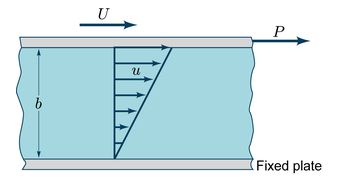
\includegraphics[width=0.5\textwidth]{1-6-1.png}
\end{center}
\textbf{Solution}
\begin{itemize}
\item The shear stress between the two parallel plates is
\[
\tau=\mu\frac{du}{dy}
=\mu\frac{U}{b}
\]
\item Thus, the viscosity of the fluid between the plates is
\[
\mu=\frac{\tau}{\left(\frac{U}{b}\right)}
=\frac{142\ \mathrm{N/m^2}}{\left(\frac{3\ \mathrm{m/s}}{0.003\ \mathrm{m}}\right)}
\]
\[
\boxed{\mu=0.142\ \frac{\mathrm{N\cdot s}}{\mathrm{m}^2}}
\]
\end{itemize}

\textbf{Problem 1.6.2}\\
A $20$-mm-diameter shaft is pulled through a cylindrical bearing as shown in the figure below. The lubricant that fills the $0.3$-mm gap between the shaft and bearing is an oil having a kinematic viscosity of $8.0\times10^{-4}\ \mathrm{m^2/s}$ and a specific gravity of $0.91$. Determine the force $P$ required to pull the shaft at a velocity of $10\ \mathrm{m/s}$. Assume the velocity distribution in the gap is linear.
\begin{center}
    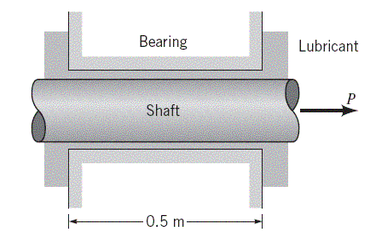
\includegraphics[width=0.5\textwidth]{1-6-2.png}
\end{center}
\textbf{Solution}
\begin{center}
    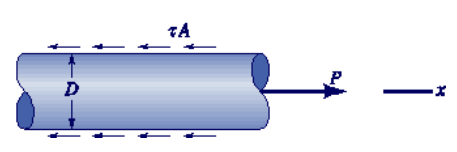
\includegraphics[width=0.5\textwidth]{1-6-2_1.png}
\end{center}
\begin{itemize}
\item From equilibrium,
\[
\sum F_x=0
\]
\[
P=\tau A
\]
\item The surface area of the shaft within the bearing is
\[
A=\pi D(\text{shaft length in bearing})=\pi Dl
\]
\item The shear stress is
\[
\tau=\mu\frac{\text{velocity of shaft}}{\text{gap width}}
=\mu\frac{V}{b}
\]
\item Thus,
\[
P=\left(\mu\frac{V}{b}\right)(\pi Dl)
=\left(\nu\rho\frac{V}{b}\right)(\pi Dl)
\]
\item Since
\[
\mu=\nu\rho=\nu(SG)\left(\rho_{\mathrm{H_2O}@4^\circ\mathrm{C}}\right)
\]
\[
P=\frac{\left(8.0\times10^{-4}\ \mathrm{m^2/s}\right)\left(0.91\times10^3\ \mathrm{kg/m^3}\right)\left(10\ \mathrm{m/s}\right)(\pi)(0.020\ \mathrm{m})(0.5\ \mathrm{m})}{0.0003\ \mathrm{m}}
\]
\[
=762\ \frac{\mathrm{kg\cdot m}}{\mathrm{s^2}}\left(\frac{1\ \mathrm{N\cdot s^2}}{1\ \mathrm{kg\cdot m}}\right)
\]
\[
\boxed{P=762\ \mathrm{N}}
\]
\end{itemize}

\textbf{Problem 1.6.3}\\
A $9$-kg block slides down a smooth inclined surface as shown in the figure below. Assume the velocity distribution in the gap is linear, the area of the block in contact with the oil is $0.3\ \mathrm{m^2}$, and $\alpha=24^\circ$. Determine the terminal velocity of the block if the gap between the block and the surface is $0.2$ mm and contains SAE 30 oil at $15.6^\circ\mathrm{C}$.
\begin{center}
    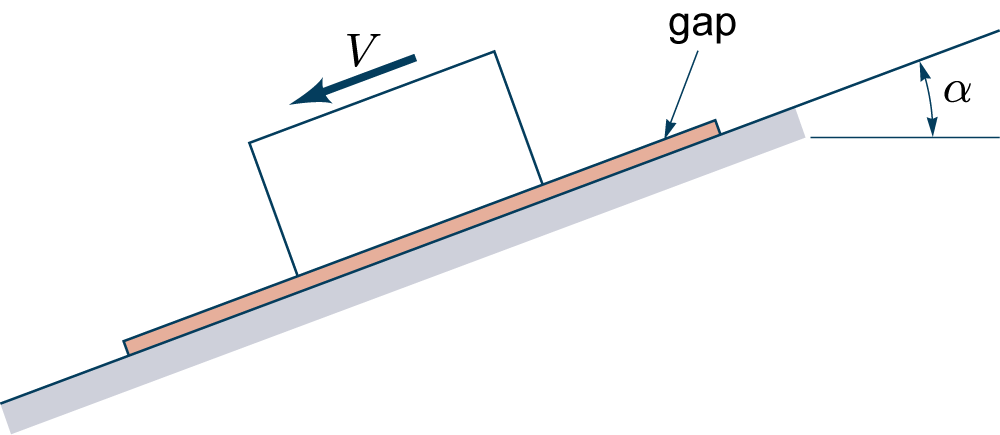
\includegraphics[width=0.5\textwidth]{1-6-3.png}
\end{center}
\textbf{Solution}
\begin{center}
    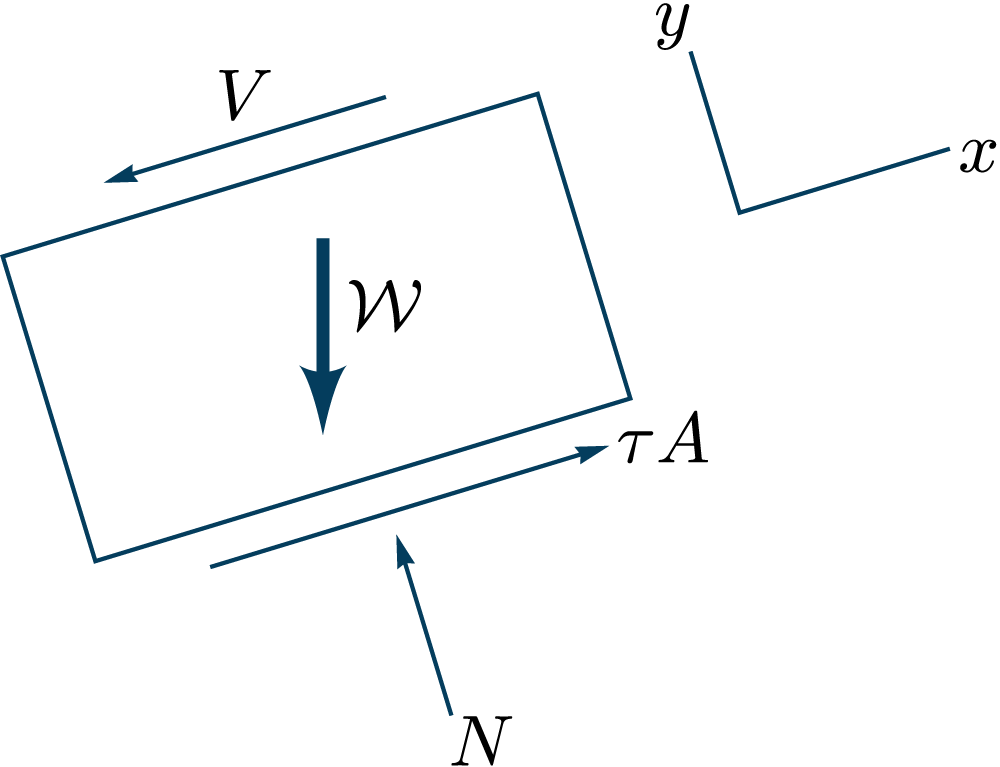
\includegraphics[width=0.3\textwidth]{1-6-3_1.png}
\end{center}
\begin{itemize}
\item Since the velocity of the block is constant,
\[
\sum F_x=0=\tau A-W\sin\alpha
\]
\[
\tau A=W\sin\alpha
\]
\item Since the velocity profile is linear and the fluid is Newtonian,
\[
\tau=\mu\frac{du}{dy}
=\mu\frac{\text{velocity}}{\text{film thickness}}
=\mu\frac{V}{b}
\]
\item Substituting the equation for $\tau$ into the force balance,
\[
\mu\frac{V}{b}A=W\sin\alpha
=mg\sin\alpha
\]
\item For SAE 30 oil at $15.6^\circ\mathrm{C}$,
\[
\mu=0.38\ \frac{\mathrm{N\cdot s}}{\mathrm{m^2}}
\]
\item Thus, the terminal velocity is
\[
V=\frac{bmg\sin\alpha}{\mu A}
=\frac{(0.0002\ \mathrm{m})(9\ \mathrm{kg})(9.81\ \mathrm{m/s^2})(\sin24^\circ)}{\left(0.38\ \mathrm{N\cdot s/m^2}\right)(0.3\ \mathrm{m^2})}
\left(\frac{1\ \mathrm{N\cdot s^2}}{1\ \mathrm{kg\cdot m}}\right)
\]
\[
\boxed{V=0.0630\ \mathrm{m/s}}
\]
\end{itemize}

\begin{center}
    {\LARGE\bfseries HW 2\par}
\end{center}
\section*{\fbox{1.7 Compressibility of fluids}}
\textbf{Problem 1.7.1}\\
A sound wave is observed to travel through a liquid with a speed of $1550\ \mathrm{m/s}$. The specific gravity of the liquid is $1.3$. Determine the bulk modulus for the liquid.\\\\
\textbf{Solution}
\begin{itemize}
\item The speed of sound is
\[
c=\sqrt{\frac{E_v}{\rho}}
\]
where
\[
\rho=SG\,\rho_{\mathrm{H_2O}}
\]
\item Thus,
\[
E_v=c^2\rho=c^2(SG)\rho_{\mathrm{H_2O}}
\]
\[
=(1550\ \mathrm{m/s})^2(1.3)(999\ \mathrm{kg/m^3})
\]
\[
\boxed{E_v=3.12\times10^9\ \mathrm{N/m^2}}
\]
\end{itemize}
\textbf{Problem 1.7.2}\\
The speed of sound in liquids is $c=\sqrt{E_v/\rho}$. Determine the speed of sound in (a) SAE 30 oil at $15.6^\circ\mathrm{C}$ and (b) glycerin at $68^\circ\mathrm{F}$.\\\\
\textbf{Solution}
\begin{itemize}
\item The speed of sound in liquids is
\[
c=\sqrt{\frac{E_v}{\rho}}
\]
\item[(a)] For SAE 30 oil at $15.6^\circ\mathrm{C}$,
\[
E_v=1.5\times10^9\ \mathrm{N/m^2},\qquad \rho=912\ \mathrm{kg/m^3}
\]
\[
c=\sqrt{\frac{1.5\times10^9\ \mathrm{N/m^2}}{912\ \mathrm{kg/m^3}}}
\]
\[
\boxed{c=1280\ \mathrm{m/s}}
\]
\item[(b)] For glycerin at $68^\circ\mathrm{F}$,
\[
E_v=6.56\times10^5\ \mathrm{lb/in^2},\qquad \rho=2.44\ \mathrm{slugs/ft^3}
\]
\[
c=\sqrt{\frac{\left(6.56\times10^5\ \mathrm{lb/in^2}\right)\left(\frac{144\ \mathrm{in^2}}{1\ \mathrm{ft^2}}\right)\left(\frac{1\ \mathrm{slug\cdot ft}}{1\ \mathrm{lb}}\right)}{2.44\ \mathrm{slugs/ft^3}}}
\]
\[
\boxed{c=6220\ \mathrm{ft/s}}
\]
\end{itemize}
\textbf{Problem 1.7.3}\\
Air is enclosed by a rigid cylinder containing a piston. A pressure gage attached to the cylinder indicates an initial reading of $35\ \mathrm{psig}$. Determine the reading on the pressure gage when the piston has compressed the air to one-fifth of its original volume. Assume the compression process to be isothermal and the local atmospheric pressure to be $14.7\ \mathrm{psi}$.\\\\
\textbf{Solution}
\begin{itemize}
\item For isothermal compression,
\[
\frac{p}{\rho}=\text{constant}
\]
so
\[
\frac{p_i}{\rho_i}=\frac{p_f}{\rho_f}
\]
\item Since the mass of air is constant inside the rigid cylinder,
\[
\rho=\frac{\text{mass}}{\text{volume}}
\]
\[
\frac{\rho_f}{\rho_i}=\frac{\text{initial volume}}{\text{final volume}}=5
\]
\item Therefore,
\[
p_f=5(35+14.7)\ \mathrm{psi\ (abs)}
=249\ \mathrm{psi\ (abs)}
\]
\item Converting back to gage pressure,
\[
p_f=(249-14.7)\ \mathrm{psi}
\]
\[
\boxed{p_f=234\ \mathrm{psi\ (gage)}}
\]
\end{itemize}

\section*{\fbox{1.9: Surface tension}}
\textbf{Problem 1.9.1}\\
When a $5$-mm-diameter tube is inserted into a liquid in an open tank, the liquid is observed to rise $16$ mm above the free surface of the liquid. The contact angle between the liquid and the tube is zero, and the specific weight of the liquid is $1.2\times10^4\ \mathrm{N/m^3}$. Determine the surface tension for the liquid.\\\\
\textbf{Solution}
\begin{itemize}
\item The capillary rise in a tube is
\[
h=\frac{2\sigma\cos\theta}{\gamma R}
\]
\item Solving for the surface tension,
\[
\sigma=\frac{\gamma hR}{2\cos\theta}
\]
\item Since $\theta=0^\circ$ and
\[
R=\frac{5\ \mathrm{mm}}{2}
\]
\[
\sigma=\frac{\left(1.2\times10^4\ \mathrm{N/m^3}\right)\left[(16\ \mathrm{mm})\left(\frac{1\ \mathrm{m}}{1000\ \mathrm{mm}}\right)\right]\left[\left(\frac{5\ \mathrm{mm}}{2}\right)\left(\frac{1\ \mathrm{m}}{1000\ \mathrm{mm}}\right)\right]}{2\cos0^\circ}
\]
\[
\boxed{\sigma=0.240\ \mathrm{N/m}}
\]
\end{itemize}
\textbf{Problem 1.9.2}\\
A $0.125$-in.-diameter glass tube is inserted into an open tank containing water at $40^\circ\mathrm{F}$. The contact angle between the liquid and the tube is zero.
\begin{itemize}
\item[(a)] Determine the height that the liquid will rise in the $0.125$-in.-diameter glass tube.
\item[(b)] Determine the height the liquid will rise in the glass tube if the diameter is reduced to $0.0115$ in.
\end{itemize}
\textbf{Solution}
\begin{itemize}
\item The capillary rise in a tube is
\[
h=\frac{2\sigma\cos\theta}{\gamma R}
\]
\item For water at $40^\circ\mathrm{F}$,
\[
\sigma=5.13\times10^{-3}\ \mathrm{lb/ft},\qquad \gamma=62.43\ \mathrm{lb/ft^3}
\]
\item[(a)] For the $0.125$-in.-diameter tube,
\[
h=\frac{2\left(5.13\times10^{-3}\ \mathrm{lb/ft}\right)(\cos0^\circ)}{\left(62.43\ \mathrm{lb/ft^3}\right)\left[\left(\frac{0.125\ \mathrm{in.}}{2}\right)\left(\frac{1\ \mathrm{ft}}{12\ \mathrm{in.}}\right)\right]}
\]
\[
=3.16\times10^{-2}\ \mathrm{ft}\left(\frac{12\ \mathrm{in.}}{1\ \mathrm{ft}}\right)
\]
\[
\boxed{h=0.379\ \mathrm{in.}}
\]
\item[(b)] For the $0.0115$-in.-diameter tube,
\[
h=\frac{2\left(5.13\times10^{-3}\ \mathrm{lb/ft}\right)(\cos0^\circ)}{\left(62.43\ \mathrm{lb/ft^3}\right)\left[\left(\frac{0.0115\ \mathrm{in.}}{2}\right)\left(\frac{1\ \mathrm{ft}}{12\ \mathrm{in.}}\right)\right]}
\]
\[
=3.43\times10^{-1}\ \mathrm{ft}\left(\frac{12\ \mathrm{in.}}{1\ \mathrm{ft}}\right)
\]
\[
\boxed{h=4.12\ \mathrm{in.}}
\]
\end{itemize}

\section*{\fbox{2.3: Pressure variation in a fluid at rest }}
\textbf{Problem 2.3.1}\\
The basic elements of a hydraulic press are shown in the figure below. A force, $F_1$, is applied to the plunger through a lever mechanism having a mechanical advantage of $7$ to $1$. The plunger has an area of $2\ \mathrm{in.^2}$, and the large piston has an area of $180\ \mathrm{in.^2}$. Neglect the hydrostatic pressure variation. Determine the load, $F_2$, that can be raised by a force of $34\ \mathrm{lb}$ applied to the lever mechanism.
\begin{center}
    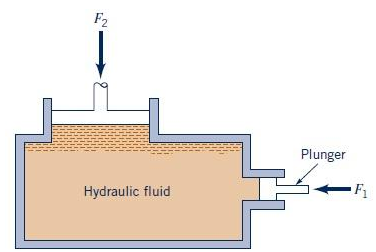
\includegraphics[width=0.5\textwidth]{2-3-1.png}
\end{center}
\textbf{Solution}
\begin{itemize}
\item A force of $34\ \mathrm{lb}$ applied to the lever mechanism results in a plunger force of
\[
F_1=(7)(34\ \mathrm{lb})
=238\ \mathrm{lb}
\]
\item The force acting on the plunger is $F_1=pA_1$ and the force acting on the large piston is $F_2=pA_2$. Since $p$ is constant throughout the hydraulic press,
\[
\frac{F_1}{A_1}=\frac{F_2}{A_2}
\]
\item Thus,
\[
F_2=\frac{A_2}{A_1}F_1
=\left(\frac{180\ \mathrm{in.^2}}{2\ \mathrm{in.^2}}\right)(238\ \mathrm{lb})
\]
\[
\boxed{F_2=21400\ \mathrm{lb}}
\]
\end{itemize}
\textbf{Problem 2.3.2}
\begin{itemize}
\item[(a)] A $2$-m-diameter vertical cylindrical tank is filled with water at $10^\circ\mathrm{C}$ to a depth of $8\ \mathrm{m}$. The rest of the tank is filled with air at atmospheric pressure. Assume $\gamma=9.804\ \mathrm{kN/m^3}$. Determine the absolute pressure at the bottom of the tank.
\item[(b)] An unknown immiscible liquid seeps into the bottom of an open oil tank. The depth of the unknown liquid is $1.5\ \mathrm{m}$ and the depth of the gasoline floating on top is $10\ \mathrm{m}$. The specific weight of gasoline is $\gamma=6.67\ \mathrm{kN/m^3}$. A pressure gage connected to the bottom of the tank reads $81\ \mathrm{kPa}$. Determine the specific gravity of the unknown liquid.
\end{itemize}
\textbf{Solution}
\begin{itemize}
\item[(a)] The absolute pressure at the bottom of the tank is
\[
p=p_{\mathrm{atm}}+\gamma h
\]
\[
=101\ \mathrm{kPa}+\left(9.804\ \mathrm{kN/m^3}\right)(8\ \mathrm{m})
\]
\[
\boxed{p=179\ \mathrm{kPa}}
\]
\item[(b)] The gage pressure at the bottom of the tank is
\[
p_{\mathrm{bottom}}=\gamma_k h_k+\gamma_u h_u
\]
where $k$ represents the known liquid, gasoline, and $u$ represents the unknown liquid.
\item Thus, the specific weight of the unknown liquid is
\[
\gamma_u=\frac{p_{\mathrm{bottom}}-\gamma_k h_k}{h_u}
\]
\[
=\frac{81\times10^3\ \mathrm{N/m^2}-\left(6.67\times10^3\ \mathrm{N/m^3}\right)(10\ \mathrm{m})}{1.5\ \mathrm{m}}
\]
\[
=9.5\times10^3\ \mathrm{N/m^3}
\]
\item Finally, the specific gravity of the unknown liquid is
\[
SG=\frac{\gamma_u}{\gamma_{\mathrm{H_2O}@4^\circ\mathrm{C}}}
=\frac{9.5\times10^3\ \mathrm{N/m^3}}{9.81\times10^3\ \mathrm{N/m^3}}
\]
\[
\boxed{SG=0.97}
\]
\end{itemize}
\newpage
\textbf{Problem 2.3.3}\\
There is a column that contains SAE 30 oil.
\begin{itemize}
\item[(a)] What is the relation between the pressure $p$, the height of column $h$, and specific weight $\gamma$?
\item[(b)] How high a column of SAE 30 oil would be required to give the same pressure as $600\ \mathrm{mm\ Hg}$?
\end{itemize}
\textbf{Solution}
\begin{itemize}
\item[(a)] The pressure due to a fluid column is
\[
\boxed{p=\gamma h}
\]
\item[(b)] For the pressures to be equal,
\[
p_{\mathrm{Hg}}=p_{\mathrm{oil}}
\]
\[
\gamma_{\mathrm{Hg}}h_{\mathrm{Hg}}=\gamma_{\mathrm{oil}}h_{\mathrm{oil}}
\]
\item Thus,
\[
h_{\mathrm{oil}}=\frac{\gamma_{\mathrm{Hg}}}{\gamma_{\mathrm{oil}}}h_{\mathrm{Hg}}
=\left(\frac{133\ \mathrm{kN/m^3}}{8.95\ \mathrm{kN/m^3}}\right)(0.600\ \mathrm{m})
\]
\[
\boxed{h_{\mathrm{oil}}=8.9\ \mathrm{m}}
\]
\end{itemize}

\section*{\fbox{2.4: Standard atmosphere}}
\textbf{Problem 2.4.1}\\
Assume that a person skiing high in the mountains at an altitude of $13500\ \mathrm{ft}$ takes in the same volume of air with each breath as she does while walking at sea level. Assume that the air composition, i.e., the percentage of air that is oxygen, is the same at sea level as it is at $13500\ \mathrm{ft}$. Determine the ratio of the mass of oxygen inhaled for each breath at this high altitude compared to that at sea level.\\\\
\textbf{Solution}
\begin{itemize}
\item Let $(\ )_0$ denote sea level and $(\ )_{13}$ denote $13500\ \mathrm{ft}$ altitude.
\item Since
\[
m=\rho V
\]
and the volume of air inhaled is the same at both elevations,
\[
m_0=\rho_0V_0,\qquad m_{13}=\rho_{13}V_{13},\qquad V_0=V_{13}
\]
\[
\frac{m_{13}}{m_0}
=\frac{\rho_{13}V_{13}}{\rho_0V_0}
=\frac{\rho_{13}}{\rho_0}
\]
\item At sea level,
\[
\rho_0=2.377\times10^{-3}\ \frac{\mathrm{slugs}}{\mathrm{ft^3}}
\]
\item Interpolate to find the density at $13500\ \mathrm{ft}$. At $10000\ \mathrm{ft}$,
\[
\rho_1=1.756\times10^{-3}\ \frac{\mathrm{slugs}}{\mathrm{ft^3}}
\]
and at $15000\ \mathrm{ft}$,
\[
\rho_2=1.496\times10^{-3}\ \frac{\mathrm{slugs}}{\mathrm{ft^3}}
\]
\[
\rho_{13}
=\rho_1+\left(\frac{h_{13}-h_1}{h_2-h_1}\right)(\rho_2-\rho_1)
\]
\[
=1.756\times10^{-3}
+\left(\frac{13500-10000}{15000-10000}\right)
\left(1.496\times10^{-3}-1.756\times10^{-3}\right)
\]
\[
=1.574\times10^{-3}\ \frac{\mathrm{slugs}}{\mathrm{ft^3}}
\]
\item Thus,
\[
\frac{m_{13}}{m_0}
=\frac{1.574\times10^{-3}}{2.377\times10^{-3}}
=0.662
\]
\[
\boxed{\frac{m_{13}}{m_0}=66.2\%}
\]
\end{itemize}
\section*{\fbox{2.5: Measurement of pressure}}
\textbf{Problem 2.5.1}
\begin{itemize}
    \item[(a)] Bourdon gages are commonly used to measure pressure. On the suction side of a pump, a Bourdon pressure gage reads $35\ \mathrm{kPa}$ vacuum. Determine the corresponding absolute pressure if the local atmospheric pressure is $95\ \mathrm{kPa}$ (abs).\\\\
\textbf{Solution}
\begin{itemize}
\item The gage pressure is negative in a vacuum. Thus, the absolute pressure is
\[
p_{\mathrm{abs}}=p_{\mathrm{gage}}+p_{\mathrm{atm}}
=-35\ \mathrm{kPa}+95\ \mathrm{kPa}
\]
\[
\boxed{p_{\mathrm{abs}}=60\ \mathrm{kPa}\ (\mathrm{abs})}
\]
\end{itemize}
    \item[(b)] On the suction side of a pump, a Bourdon pressure gage reads $46\ \mathrm{kPa}$ vacuum when the local atmospheric pressure is $100\ \mathrm{kPa}$ (abs). Determine the gage reading if the local atmospheric pressure decreases to $90\ \mathrm{kPa}$ (abs).\\\\
\textbf{Solution}
\begin{itemize}
\item The absolute pressure is
\[
p_{\mathrm{abs}}=p_{\mathrm{gage}}+p_{\mathrm{atm}}
\]
\item Assuming the absolute pressure remains constant,
\[
(p_{\mathrm{gage}}+p_{\mathrm{atm}})_i=(p_{\mathrm{gage}}+p_{\mathrm{atm}})_f
\]
\item Since the initial gage pressure is negative in a vacuum,
\[
p_{\mathrm{gage},f}=p_{\mathrm{gage},i}+p_{\mathrm{atm},i}-p_{\mathrm{atm},f}
=-46\ \mathrm{kPa}+100\ \mathrm{kPa}-90\ \mathrm{kPa}
\]
\[
\boxed{p_{\mathrm{gage},f}=-36\ \mathrm{kPa}}
\]
\end{itemize}
    \item[(c)] When a Bourdon pressure gage is attached to the closed water tank in the figure below, the gage reads $8\ \mathrm{psi}$ (gage). Assume that the standard atmospheric pressure is $14.7\ \mathrm{psia}$ and that the specific weight of water is $62.4\ \mathrm{lb/ft^3}$. Determine the absolute air pressure $p_{\mathrm{air}}$ in the tank.
\begin{center}
    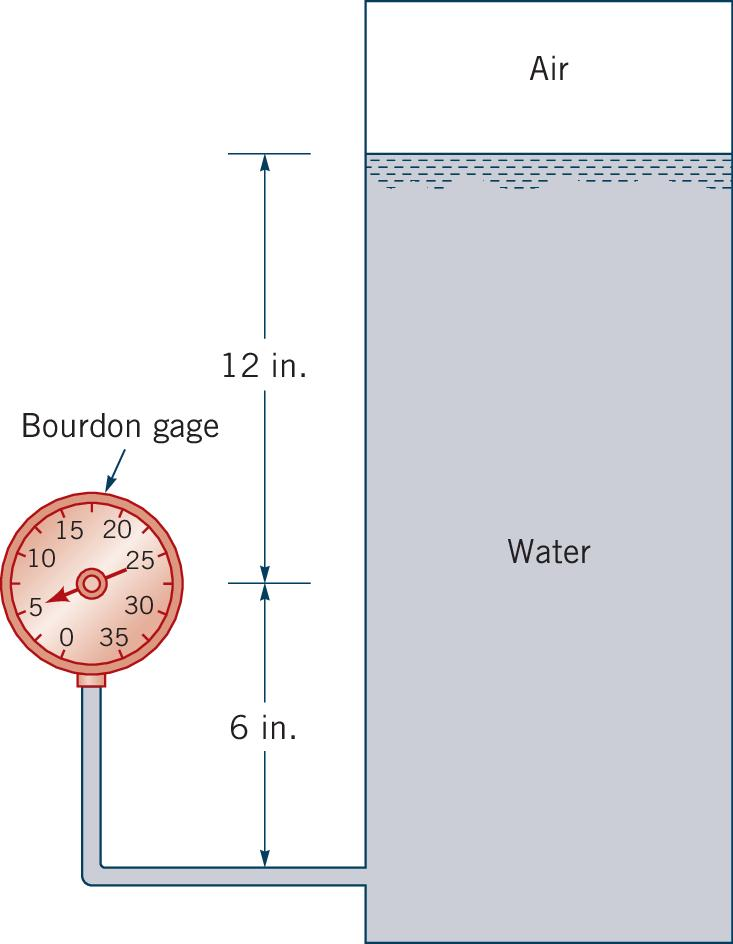
\includegraphics[width=0.5\textwidth]{2-5-3.jpg}
\end{center}
\textbf{Solution}
\begin{itemize}
\item At the Bourdon gage, the absolute pressure is
\[
p=\gamma h+p_{\mathrm{air}}
\]
\item Thus,
\[
p_{\mathrm{gage}}+p_{\mathrm{atm}}=\gamma h+p_{\mathrm{air}}
\]
\[
p_{\mathrm{air}}=(p_{\mathrm{gage}}+p_{\mathrm{atm}})-\gamma h
\]
\item Substituting the known values,
\[
p_{\mathrm{air}}
=\left(8\ \mathrm{lb/in.^2}+14.7\ \mathrm{lb/in.^2}\right)
-\left(62.4\ \mathrm{lb/ft^3}\right)
\left(\frac{1\ \mathrm{ft}}{12\ \mathrm{in.}}\right)^3
(12\ \mathrm{in.})
\]
\[
\boxed{p_{\mathrm{air}}=22.3\ \mathrm{psia}}
\]
\end{itemize}
\end{itemize}

\section*{\fbox{2.6: Manometry}}
\textbf{Problem 2.6.1}\\
The atmospheric pressure is $92\ \mathrm{kPa}$ (abs). The vapor pressure and specific weight for mercury, water, and ethyl alcohol are given below.
\[
\begin{array}{c|c|c}
\text{Fluid} & p_v\ (\mathrm{N/m^2}) & \gamma\ (\mathrm{kN/m^3})\\
\hline
\text{Mercury} & 0.16 & 133\\
\text{Water} & 1770 & 9.80\\
\text{Ethyl alcohol} & 5900 & 7.74
\end{array}
\]
Determine the height of the fluid column in a barometer containing (a) mercury, (b) water, and (c) ethyl alcohol, both neglecting vapor pressure and including vapor pressure.\\\\
\textbf{Solution}
\begin{itemize}
\item The barometer relation neglecting vapor pressure is
\[
p_{\mathrm{atm}}=\gamma h
\]
\[
h=\frac{p_{\mathrm{atm}}}{\gamma}
\]
\item When vapor pressure is included,
\[
p_{\mathrm{atm}}=\gamma h+p_v
\]
\[
h=\frac{p_{\mathrm{atm}}-p_v}{\gamma}
\]
\item[(a)] For mercury:
\[
h_{\mathrm{Hg}}=\frac{92\times10^3\ \mathrm{N/m^2}}{133\times10^3\ \mathrm{N/m^3}}
\]
\[
\boxed{h_{\mathrm{Hg}}=0.692\ \mathrm{m}}\qquad\text{(neglecting vapor pressure)}
\]
\[
h_{\mathrm{Hg}}=\frac{92\times10^3\ \mathrm{N/m^2}-0.16\ \mathrm{N/m^2}}{133\times10^3\ \mathrm{N/m^3}}
\]
\[
\boxed{h_{\mathrm{Hg}}=0.692\ \mathrm{m}}\qquad\text{(including vapor pressure)}
\]
\item[(b)] For water:
\[
h_{\mathrm{water}}=\frac{92\times10^3\ \mathrm{N/m^2}}{9.80\times10^3\ \mathrm{N/m^3}}
\]
\[
\boxed{h_{\mathrm{water}}=9.39\ \mathrm{m}}\qquad\text{(neglecting vapor pressure)}
\]
\[
h_{\mathrm{water}}=\frac{92\times10^3\ \mathrm{N/m^2}-1770\ \mathrm{N/m^2}}{9.80\times10^3\ \mathrm{N/m^3}}
\]
\[
\boxed{h_{\mathrm{water}}=9.21\ \mathrm{m}}\qquad\text{(including vapor pressure)}
\]
\item[(c)] For ethyl alcohol:
\[
h_{\mathrm{alcohol}}=\frac{92\times10^3\ \mathrm{N/m^2}}{7.74\times10^3\ \mathrm{N/m^3}}
\]
\[
\boxed{h_{\mathrm{alcohol}}=11.9\ \mathrm{m}}\qquad\text{(neglecting vapor pressure)}
\]
\[
h_{\mathrm{alcohol}}=\frac{92\times10^3\ \mathrm{N/m^2}-5900\ \mathrm{N/m^2}}{7.74\times10^3\ \mathrm{N/m^3}}
\]
\[
\boxed{h_{\mathrm{alcohol}}=11.1\ \mathrm{m}}\qquad\text{(including vapor pressure)}
\]
\end{itemize}

\textbf{Problem 2.6.2}\\
The closed tank in the figure is filled with water.
\begin{center}
    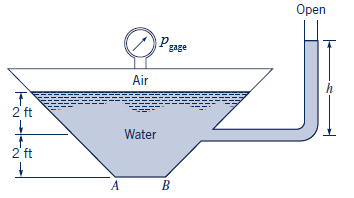
\includegraphics[width=0.5\textwidth]{2-6-2.png}
\end{center}
\begin{itemize}
\item[(a)] The pressure gage on the tank reads $p_{\mathrm{gage}}=7.80\ \mathrm{psi}$. Determine the height, $h$, in the open water column.
\item[(b)] If the tank has a column height $h=5\ \mathrm{ft}$ and the pressure gage reads $p_{\mathrm{gage}}=7.90\ \mathrm{psi}$, determine the gage pressure acting on the bottom tank surface $AB$.
\item[(c)] If the tank has a column height $h=7\ \mathrm{ft}$ and the pressure gage reads $p_{\mathrm{gage}}=7.70\ \mathrm{psi}$, determine the absolute pressure of the air in the top of the tank if the local atmospheric pressure is $14.7\ \mathrm{psia}$.
\end{itemize}
\textbf{Solution}
\begin{itemize}
\item[(a)] Applying the pressure relation between the water surface in the open tube and the air pressure in the tank,
\[
\gamma h-\gamma(2\ \mathrm{ft})=p_{\mathrm{air}}
\]
\[
h=\frac{p_{\mathrm{air}}+\gamma(2\ \mathrm{ft})}{\gamma}
=\frac{\left(7.80\ \mathrm{lb/in.^2}\right)\left(\frac{144\ \mathrm{in.^2}}{1\ \mathrm{ft^2}}\right)+\left(62.4\ \mathrm{lb/ft^3}\right)(2\ \mathrm{ft})}{62.4\ \mathrm{lb/ft^3}}
\]
\[
\boxed{h=20.0\ \mathrm{ft}}
\]
\item[(b)] The gage pressure at the bottom of the tank is
\[
p_{AB}=\gamma(4\ \mathrm{ft})+p_{\mathrm{air}}
=\left[\left(62.4\ \mathrm{lb/ft^3}\right)(4\ \mathrm{ft})\right]\left(\frac{1\ \mathrm{ft^2}}{144\ \mathrm{in.^2}}\right)+7.90\ \mathrm{lb/in.^2}
\]
\[
\boxed{p_{AB}=9.63\ \mathrm{psi}}
\]
\item[(c)] The absolute pressure of the air is
\[
p_{\mathrm{air}}=p_{\mathrm{gage}}+p_{\mathrm{atm}}
=7.70\ \mathrm{psi}+14.7\ \mathrm{psia}
\]
\[
\boxed{p_{\mathrm{air}}=22.4\ \mathrm{psia}}
\]
\end{itemize}

\textbf{Problem 2.6.3(a)}\\
The U-tube manometer shown in the figure below has two fluids, water and oil $(SG=0.80)$. The height of the oil column is $h_0=16\ \mathrm{cm}$. Find the height difference between the free oil surface and the free water surface with no applied pressure difference.
\begin{center}
    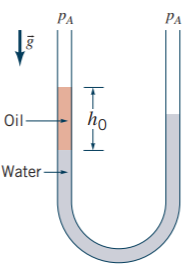
\includegraphics[width=0.3\textwidth]{2-6-3a.png}
\end{center}
\textbf{Solution}
\begin{itemize}
\item Applying the manometer rule,
\[
p_A+\rho_o g h_0-\rho_w g h_w=p_A
\]
\item Solving for the height difference between the two water levels,
\[
h_w=h_0\left(\frac{\rho_o}{\rho_w}\right)
=h_0SG_o
\]
\[
=(16\ \mathrm{cm})(0.80)
=12.8\ \mathrm{cm}
\]
\item Thus, the height difference between the free oil surface and the free water surface is
\[
\Delta h=h_0-h_w
=16\ \mathrm{cm}-12.8\ \mathrm{cm}
\]
\[
\boxed{\Delta h=3.2\ \mathrm{cm}}
\]
\end{itemize}
\textbf{Problem 2.6.3(b)}\\
Two pipes are connected by a manometer, as shown in the figure below. The gage fluid has a specific gravity $SG=2.1$. Determine the pressure difference, $p_A-p_B$, between the pipes.
\begin{center}
    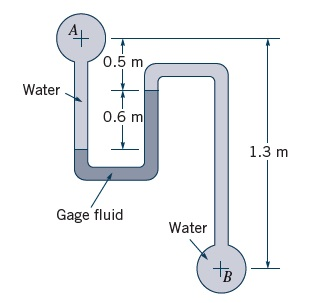
\includegraphics[width=0.5\textwidth]{2-6-3b.jpg}
\end{center}
\textbf{Solution}
\begin{itemize}
\item Applying the manometer rule between points $A$ and $B$,
\[
p_A+\gamma_{\mathrm{H_2O}}(0.5\ \mathrm{m}+0.6\ \mathrm{m})
-\gamma_{\mathrm{gage}}(0.6\ \mathrm{m})
+\gamma_{\mathrm{H_2O}}(1.3\ \mathrm{m}-0.5\ \mathrm{m})
=p_B
\]
\item Thus,
\[
p_A-p_B
=\gamma_{\mathrm{gage}}(0.6\ \mathrm{m})
-\gamma_{\mathrm{H_2O}}(0.5\ \mathrm{m}+0.6\ \mathrm{m}+1.3\ \mathrm{m}-0.5\ \mathrm{m})
\]
\[
=(2.1)\left(9.80\ \mathrm{kN/m^3}\right)(0.6\ \mathrm{m})
-\left(9.80\ \mathrm{kN/m^3}\right)(1.9\ \mathrm{m})
\]
\[
\boxed{p_A-p_B=-6.27\ \mathrm{kPa}}
\]
\end{itemize}
\textbf{Problem 2.6.3(c)}\\
A closed cylindrical tank filled with water has a hemispherical dome and is connected to an inverted piping system as shown in the figure below. The liquid in the top part of the piping system has a specific gravity of $0.5$, and the remaining parts of the system are filled with water. Assume $p_A=60\ \mathrm{kPa}$, $h_1=1\ \mathrm{m}$, $h_2=4\ \mathrm{m}$, $h_3=2\ \mathrm{m}$, and $R_1=2\ \mathrm{m}$.
\begin{center}
    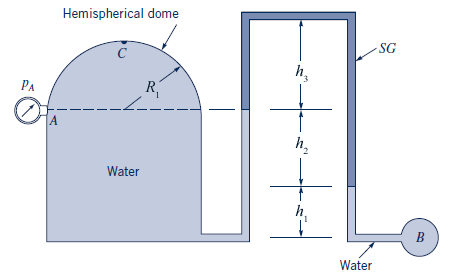
\includegraphics[width=0.6\textwidth]{2-6-3c.png}
\end{center}
\begin{itemize}
\item[(a)] Determine the pressure at point $B$.
\item[(b)] Determine the pressure head at the top of the dome, point $C$, in millimeters of mercury. Assume $\gamma_{\mathrm{Hg}}=133\ \mathrm{kN/m^3}$.
\end{itemize}
\textbf{Solution}
\begin{itemize}
\item[(a)] Applying the manometer rule between points $A$ and $B$,
\[
p_A+(SG)(\gamma_{\mathrm{H_2O}})(h_2)+\gamma_{\mathrm{H_2O}}(h_1)=p_B
\]
\[
p_B=60\times10^3\ \mathrm{Pa}
+(0.5)\left(9.80\times10^3\ \mathrm{N/m^3}\right)(4\ \mathrm{m})
+\left(9.80\times10^3\ \mathrm{N/m^3}\right)(1\ \mathrm{m})
\]
\[
=8.94\times10^4\ \mathrm{Pa}
\]
\[
\boxed{p_B=89.4\ \mathrm{kPa}}
\]
\item[(b)] Applying the pressure relation between points $A$ and $C$,
\[
p_C=p_A-\gamma_{\mathrm{H_2O}}R_1
=60\times10^3\ \mathrm{Pa}
-\left(9.80\times10^3\ \mathrm{N/m^3}\right)(2\ \mathrm{m})
\]
\[
=4.04\times10^4\ \mathrm{N/m^2}
\]
\item The pressure head in mercury is
\[
h=\frac{p_C}{\gamma_{\mathrm{Hg}}}
=\left(\frac{4.04\times10^4\ \mathrm{N/m^2}}{133\times10^3\ \mathrm{N/m^3}}\right)
\left(\frac{1000\ \mathrm{mm}}{1\ \mathrm{m}}\right)
\]
\[
\boxed{h=304\ \mathrm{mm\ Hg}}
\]
\end{itemize}

\textbf{Problem 2.6.4}\\
A U-tube manometer is connected to a closed tank containing air and water as shown in the figure below. At the closed end of the manometer, the air pressure is $18\ \mathrm{psia}$, the height of the column of the gage fluid is $h_2=4\ \mathrm{ft}$, and the depth of the gage below the free surface is $h_1=2\ \mathrm{ft}$. Assume standard atmospheric pressure and neglect the weight of the air columns in the manometer. Determine the reading on the pressure gage for a differential reading of $h_2=4\ \mathrm{ft}$ on the manometer. Express your answer in psi (gage).
\begin{center}
    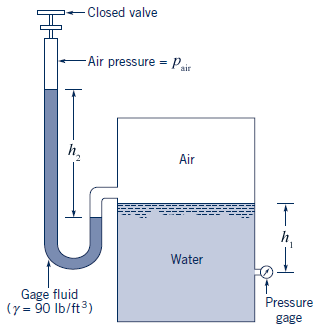
\includegraphics[width=0.5\textwidth]{2-6-4.png}
\end{center}
\textbf{Solution}
\begin{itemize}
\item The gage pressure is
\[
p_{\mathrm{gage}}=p_1+\gamma_{\mathrm{gf}}h_2+\gamma_{\mathrm{H_2O}}h_1
\]
where $p_1$ is the air pressure relative to atmospheric pressure.
\item Thus,
\[
p_1=p_{\mathrm{air}}-p_{\mathrm{atm}}
=18\ \mathrm{psi}-14.7\ \mathrm{psi}
=3.3\ \mathrm{psi}
\]
\item Substituting the known values,
\[
p_{\mathrm{gage}}
=\left(3.3\ \mathrm{lb/in.^2}\right)\left(\frac{144\ \mathrm{in.^2}}{1\ \mathrm{ft^2}}\right)
+\left(90\ \mathrm{lb/ft^3}\right)(4\ \mathrm{ft})
+\left(62.4\ \mathrm{lb/ft^3}\right)(2\ \mathrm{ft})
\]
\[
=960\ \mathrm{lb/ft^2}
\]
\[
p_{\mathrm{gage}}
=\left(960\ \mathrm{lb/ft^2}\right)\left(\frac{1\ \mathrm{ft^2}}{144\ \mathrm{in.^2}}\right)
\]
\[
\boxed{p_{\mathrm{gage}}=6.67\ \mathrm{psi}}
\]
\end{itemize}

\textbf{Problem 2.6.5}\\
For the inclined-tube manometer in the figure below, the pressure in pipe $A$ is $1.2\ \mathrm{psi}$. The fluid in both pipes $A$ and $B$ is water, and the gage fluid in the manometer has a specific gravity of $2.6$. Determine the pressure in pipe $B$ corresponding to the differential reading shown.
\begin{center}
    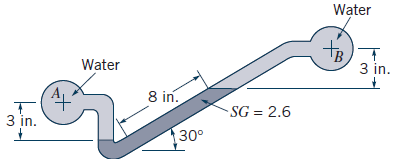
\includegraphics[width=0.5\textwidth]{2-6-5.png}
\end{center}
\textbf{Solution}
\begin{itemize}
\item Applying the manometer rule from $A$ to $B$,
\[
p_A+\gamma_{\mathrm{H_2O}}\left(\frac{3}{12}\ \mathrm{ft}\right)
-\gamma_{\mathrm{gf}}\left(\frac{8}{12}\ \mathrm{ft}\right)\sin30^\circ
-\gamma_{\mathrm{H_2O}}\left(\frac{3}{12}\ \mathrm{ft}\right)
=p_B
\]
\item The water terms cancel, so
\[
p_B=p_A-\gamma_{\mathrm{gf}}\left(\frac{8}{12}\ \mathrm{ft}\right)\sin30^\circ
\]
\item Since
\[
\gamma_{\mathrm{gf}}=(SG)\gamma_{\mathrm{H_2O}}
=(2.6)\left(62.4\ \mathrm{lb/ft^3}\right)
\]
\[
p_B
=\left(1.2\ \mathrm{lb/in.^2}\right)\left(\frac{144\ \mathrm{in.^2}}{1\ \mathrm{ft^2}}\right)
-(2.6)\left(62.4\ \mathrm{lb/ft^3}\right)\left(\frac{8}{12}\ \mathrm{ft}\right)(0.5)
\]
\[
=118.72\ \mathrm{lb/ft^2}
\]
\[
=\left(118.72\ \mathrm{lb/ft^2}\right)\left(\frac{1\ \mathrm{ft^2}}{144\ \mathrm{in.^2}}\right)
\]
\[
\boxed{p_B=0.824\ \mathrm{psi}}
\]
\end{itemize}

\begin{center}
    {\LARGE\bfseries HW 3\par}
\end{center}
\section*{\fbox{2.8 Hydrostatic force on a plane surface}}
\textbf{Problem 2.8.1(a)}\\
The weight $\mathcal{W}$ is used to hold the wall upright as shown in the figure below. The wall is $20\ \mathrm{m}$ wide. The height of the water is $h_1=7\ \mathrm{m}$, and the height between the water and the top of the rope is $h_2=5\ \mathrm{m}$. Assume $\rho=1000\ \mathrm{kg/m^3}$.
\begin{center}
    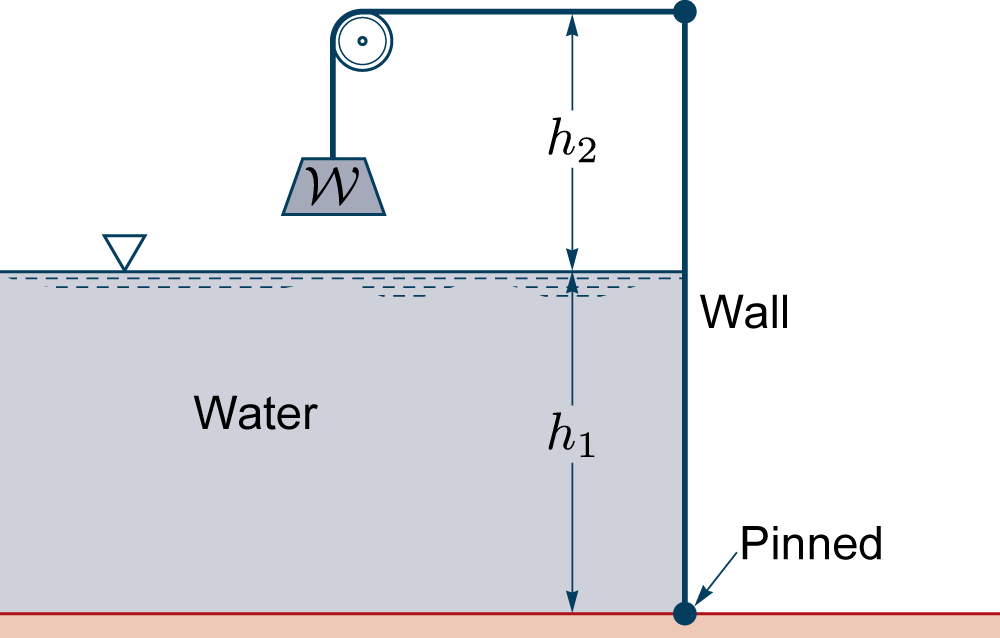
\includegraphics[width=0.5\textwidth]{2-8-1.png}
\end{center}
\begin{itemize}
\item[(a)] Determine the hydrostatic force $F_R$ acting on the wall.
\item[(b)] Determine the weight $\mathcal{W}$ needed to hold the wall upright.
\end{itemize}
\textbf{Solution}
\begin{itemize}
\item[(a)] The hydrostatic force acting on the wall is
\[
F_R=\rho g h_c A
\]
\[
=\left(1000\ \mathrm{kg/m^3}\right)\left(9.81\ \mathrm{m/s^2}\right)\left(\frac{7\ \mathrm{m}}{2}\right)\left[(7\ \mathrm{m})(20\ \mathrm{m})\right]
\]
\[
=\left(4810000\ \mathrm{kg\cdot m/s^2}\right)\left(\frac{1\ \mathrm{kN}}{1000\ \mathrm{N}}\right)
\]
\[
\boxed{F_R=4810\ \mathrm{kN}}
\]
\item[(b)] The hydrostatic force $F_R$ is located one-third of the water depth from the bottom of the water, as shown below.
\begin{center}
    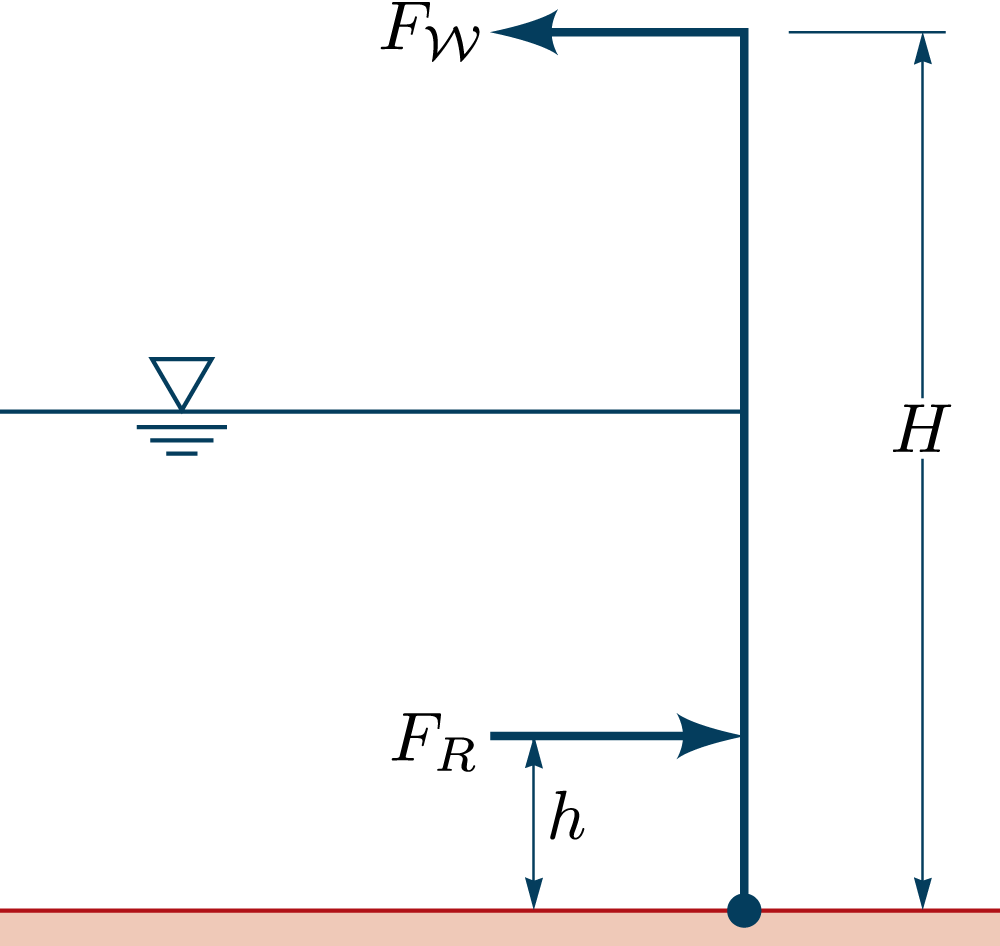
\includegraphics[width=0.3\textwidth]{2-8-1_1.png}
\end{center}
\item Thus, $F_R$ is located at a height $h$ above the pin,
\[
h=\frac{1}{3}h_1
=\frac{1}{3}(7\ \mathrm{m})
=2.33\ \mathrm{m}
\]
\item The weight force $F_W$ is located at a height
\[
H=h_1+h_2
=7\ \mathrm{m}+5\ \mathrm{m}
=12\ \mathrm{m}
\]
above the pin. Summing moments about the pinned joint,
\[
\sum M_{\mathrm{pin}}=F_WH-F_Rh=0
\]
\[
F_W=\frac{h}{H}F_R
=\frac{2.33\ \mathrm{m}}{7\ \mathrm{m}+5\ \mathrm{m}}(4810\ \mathrm{kN})
\]
\[
F_W=935\ \mathrm{kN}
\]
\item Assuming no friction between the rope and the pulley,
\[
\boxed{\mathcal{W}=F_W=935\ \mathrm{kN}}
\]
\end{itemize}

\textbf{Problem 2.8.1(b)}\\
The width of the gate in the figure below is $7$-m wide. The height of the water is $H=1.8\ \mathrm{m}$, and the height of the gate is $h=1.0\ \mathrm{m}$. Assume $\rho=1000\ \mathrm{kg/m^3}$.
\begin{center}
    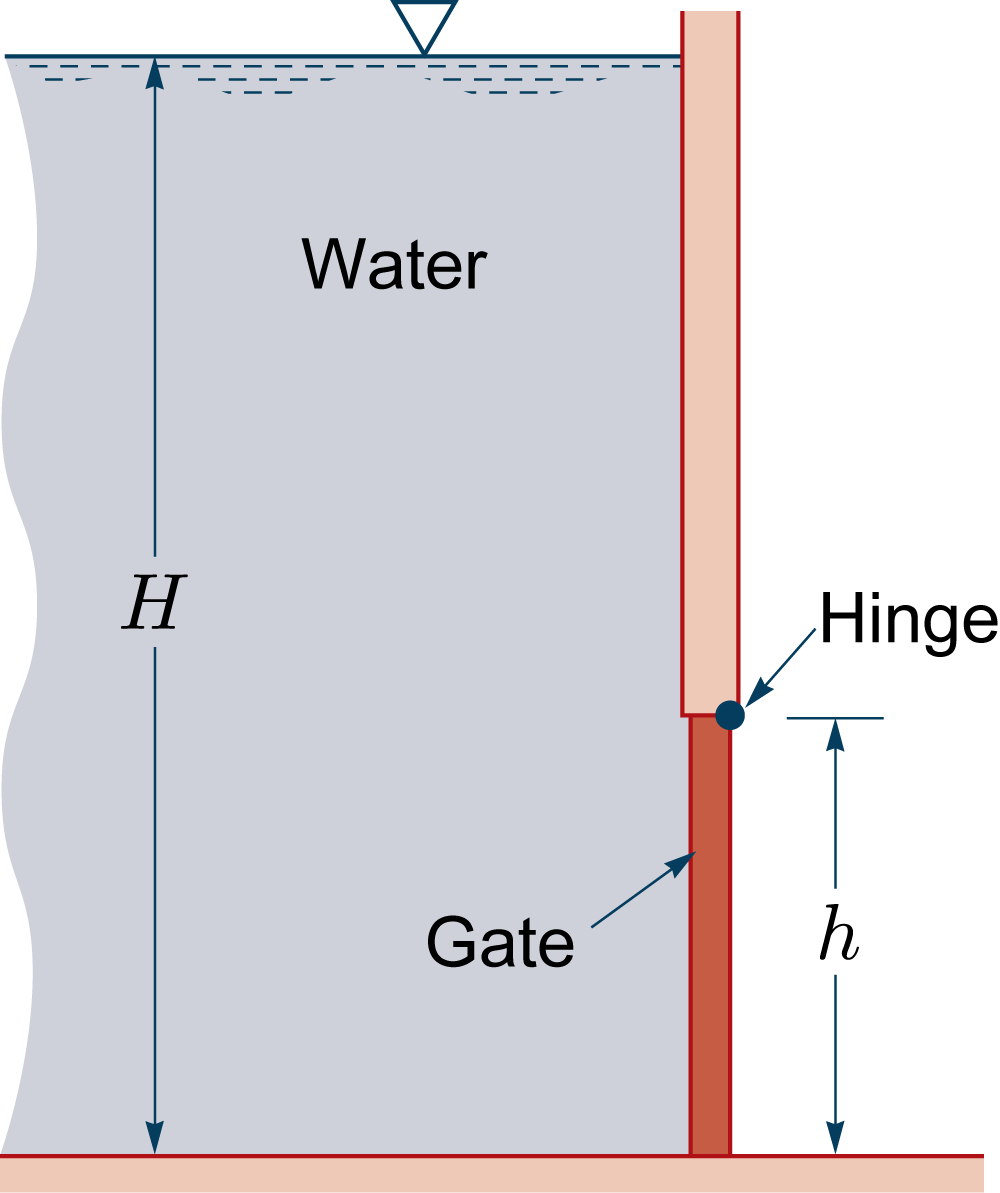
\includegraphics[width=0.3\textwidth]{2-8-1b.png}
\end{center}
\begin{itemize}
\item[(a)] Determine the direction of the force that must be applied to the bottom of the gate to keep the gate closed.
\item[(b)] Determine the magnitude of the force that must be applied to the bottom of the gate to keep the gate closed.
\end{itemize}
\textbf{Solution}
\begin{itemize}
\item[(a)] The force applied to the bottom of the gate $F_P$ must act leftwards to counter the hydrostatic force acting on the gate, as shown below.
\begin{center}
    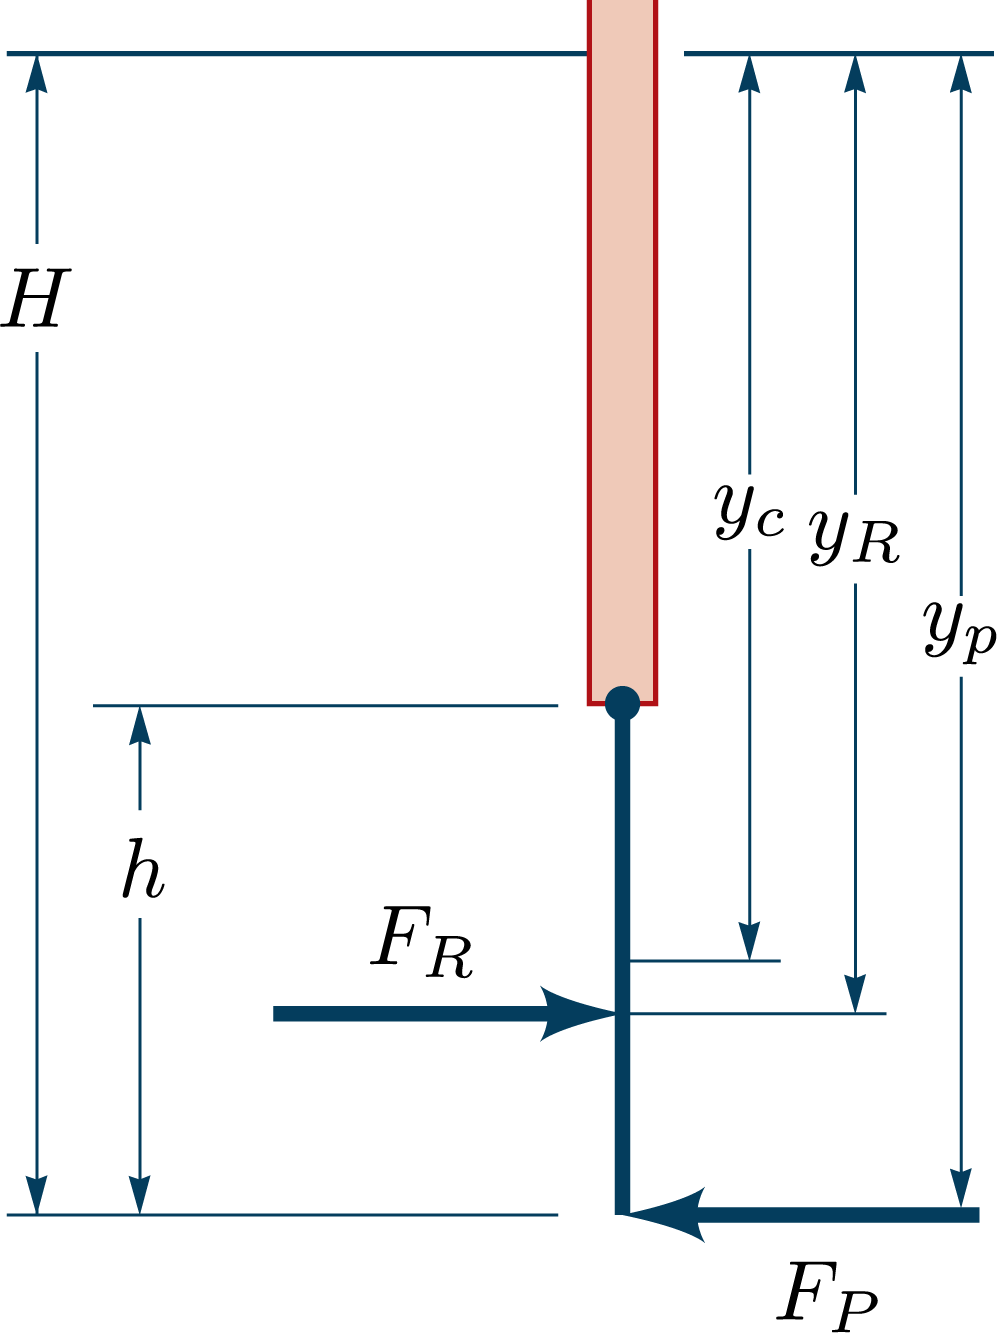
\includegraphics[width=0.3\textwidth]{2-8-1b_1.png}
\end{center}
\[
\boxed{\text{Leftwards}}
\]
\item[(b)] The hydrostatic force acting on the gate is
\[
F_R=\rho g y_cA
\]
\[
=\left(1000\ \mathrm{kg/m^3}\right)\left(9.81\ \mathrm{m/s^2}\right)(1.8\ \mathrm{m}-0.50\ \mathrm{m})[(1.0\ \mathrm{m})(7\ \mathrm{m})]
\]
\[
=\left(89300\ \mathrm{kg\cdot m/s^2}\right)\left(\frac{1\ \mathrm{kN}}{1000\ \mathrm{N}}\right)
\]
\[
F_R=89.3\ \mathrm{kN}
\]
\item The location of the hydrostatic force $F_R$ is
\[
y_R=\frac{I_{xc}}{y_cA}+y_c
\]
\[
=\frac{\frac{1}{12}(7\ \mathrm{m})(1.0\ \mathrm{m})^3}{(1.8\ \mathrm{m}-0.50\ \mathrm{m})[(1.0\ \mathrm{m})(7\ \mathrm{m})]}+(1.8\ \mathrm{m}-0.50\ \mathrm{m})
\]
\[
y_R=1.36\ \mathrm{m}
\]
\item Summing moments about the hinge,
\[
\sum M_{\mathrm{hinge}}
=F_R[y_R-(H-h)]-F_Ph=0
\]
\[
F_P=\frac{F_R[y_R-(H-h)]}{h}
\]
\[
=\frac{89.3\ \mathrm{kN}[1.36\ \mathrm{m}-(1.8\ \mathrm{m}-1.0\ \mathrm{m})]}{1.0\ \mathrm{m}}
\]
\[
\boxed{F_P=50.4\ \mathrm{kN}}
\]
\end{itemize}

\textbf{Problem 2.8.2}\\
A structure with a hatch is attached to the ground and submerged in seawater $(\gamma=10.1\ \mathrm{kN/m^3})$. The $3$-m-diameter hatch is angled at $\theta=35^\circ$ and hinged on its top edge. The hatch hinge is located at a depth of $h_1=14\ \mathrm{m}$ from the free surface. Neglect the weight of the hatch and friction in the hinge.
\begin{center}
    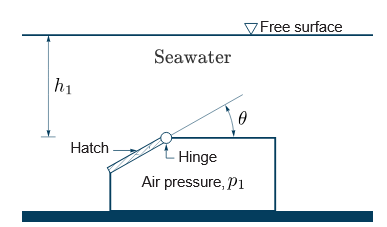
\includegraphics[width=0.5\textwidth]{2-8-2.png}
\end{center}
\begin{itemize}
\item[(a)] Calculate the resultant force $F_R$ acting on the hatch.
\item[(b)] Calculate the resultant force's $y$-coordinate $y_R$.
\item[(c)] Determine the minimum air gage pressure, $p_1$, within the container that will open the hatch.
\end{itemize}
\textbf{Solution}
\begin{itemize}
\item[(a)] The resultant force is
\[
F_R=\gamma h_cA
\]
where the centroid height $h_c$ is
\[
h_c=14\ \mathrm{m}+\frac{1}{2}(3\ \mathrm{m})\sin35^\circ
=14.9\ \mathrm{m}
\]
\[
F_R=\left(10.1\ \mathrm{kN/m^3}\right)(14.9\ \mathrm{m})\left(\frac{\pi}{4}\right)(3\ \mathrm{m})^2
\]
\[
\boxed{F_R=1064\ \mathrm{kN}}
\]
\item[(b)] The resultant force's $y$-coordinate is
\[
y_R=\frac{I_{xc}}{y_cA}+y_c
\]
where the distance to the centroid along the $y$-axis is
\[
y_c=\frac{14\ \mathrm{m}}{\sin35^\circ}+1.5\ \mathrm{m}
=25.908\ \mathrm{m}
\]
\[
y_R=\frac{\left(\frac{\pi}{4}\right)(1.5\ \mathrm{m})^4}{(25.908\ \mathrm{m})\left[\pi(1.5\ \mathrm{m})^2\right]}+25.908\ \mathrm{m}
\]
\[
\boxed{y_R=25.930\ \mathrm{m}}
\]
\item[(c)] The minimum air gage pressure $p_1$ is determined by summing moments about the hinge $H$.
\begin{center}
    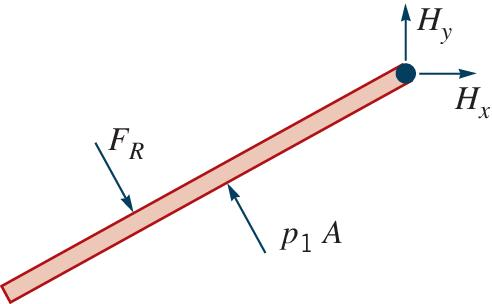
\includegraphics[width=0.4\textwidth]{2-8-2_1.jpg}
\end{center}
\[
\sum M_H=0
\]
\item The $y$-coordinate of the hinge is
\[
y_H=\frac{14\ \mathrm{m}}{\sin35^\circ}
=24.408\ \mathrm{m}
\]
\item Thus,
\[
F_R(25.930\ \mathrm{m}-24.408\ \mathrm{m})
=p_1\left[\pi(1.5\ \mathrm{m})^2\right](1.5\ \mathrm{m})
\]
\[
p_1=
\frac{(1.064\times10^6\ \mathrm{N})(25.930\ \mathrm{m}-24.408\ \mathrm{m})}
{\pi(1.5\ \mathrm{m})^2(1.5\ \mathrm{m})}
\]
\[
=1.53\times10^5\ \mathrm{Pa}
\]
\[
\boxed{p_1=153\ \mathrm{kPa}}
\]
\end{itemize}

\textbf{Problem 2.8.3}\\
A homogeneous rectangular gate is held in place by a horizontal flexible cable as shown in the figure below. Water acts against the gate, which is hinged at point $A$. Assume $\gamma=62.4\ \mathrm{lb/ft^3}$. The gate is $3$ ft wide, $8$ ft long, and weighs $800\ \mathrm{lb}$. Assume $L_1=8\ \mathrm{ft}$, $L_2=6\ \mathrm{ft}$, and $\theta=58^\circ$.
\begin{center}
    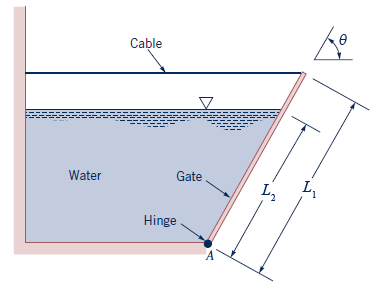
\includegraphics[width=0.5\textwidth]{2-8-3.png}
\end{center}
\begin{itemize}
\item[(a)] Determine the vertical distance from the fluid surface to the centroid of the gate, $h_c$, and the magnitude of the resultant force acting on the gate, $F_R$.
\item[(b)] Determine the second moment of area, $I_{xc}$, and the $y$ coordinate of the resultant force, $y_R$.
\item[(c)] Determine the tension in the cable, $T$.
\end{itemize}

\textbf{Solution}
\begin{itemize}
\item[(a)] The vertical distance from the fluid surface to the centroid of the gate is
\[
h_c=\frac{L_2\sin\theta}{2}
=\frac{(6\ \mathrm{ft})\sin58^\circ}{2}
\]
\[
\boxed{h_c=2.54\ \mathrm{ft}}
\]
The magnitude of the resultant force acting on the gate is
\[
F_R=\gamma h_cA
\]
\[
=\left(62.4\ \mathrm{lb/ft^3}\right)(2.54\ \mathrm{ft})[(3\ \mathrm{ft})(6\ \mathrm{ft})]
\]
\[
\boxed{F_R=2850\ \mathrm{lb}}
\]

\item[(b)] The second moment of area is
\[
I_{xc}=\frac{1}{12}wL_2^3
=\frac{1}{12}(3\ \mathrm{ft})(6\ \mathrm{ft})^3
\]
\[
\boxed{I_{xc}=54.0\ \mathrm{ft^4}}
\]
The $y$ coordinate of the centroid of the gate is
\[
y_c=\frac{L_2}{2}
=\frac{6\ \mathrm{ft}}{2}
=3.0\ \mathrm{ft}
\]
The $y$ coordinate of the resultant force is
\[
y_R=\frac{I_{xc}}{y_cA}+y_c
\]
\[
=\frac{54.0\ \mathrm{ft^4}}{(3.0\ \mathrm{ft})[(3\ \mathrm{ft})(6\ \mathrm{ft})]}+3.0\ \mathrm{ft}
\]
\[
\boxed{y_R=4.00\ \mathrm{ft}}
\]

\item[(c)] The free body diagram of the gate is shown below.
\begin{center}
    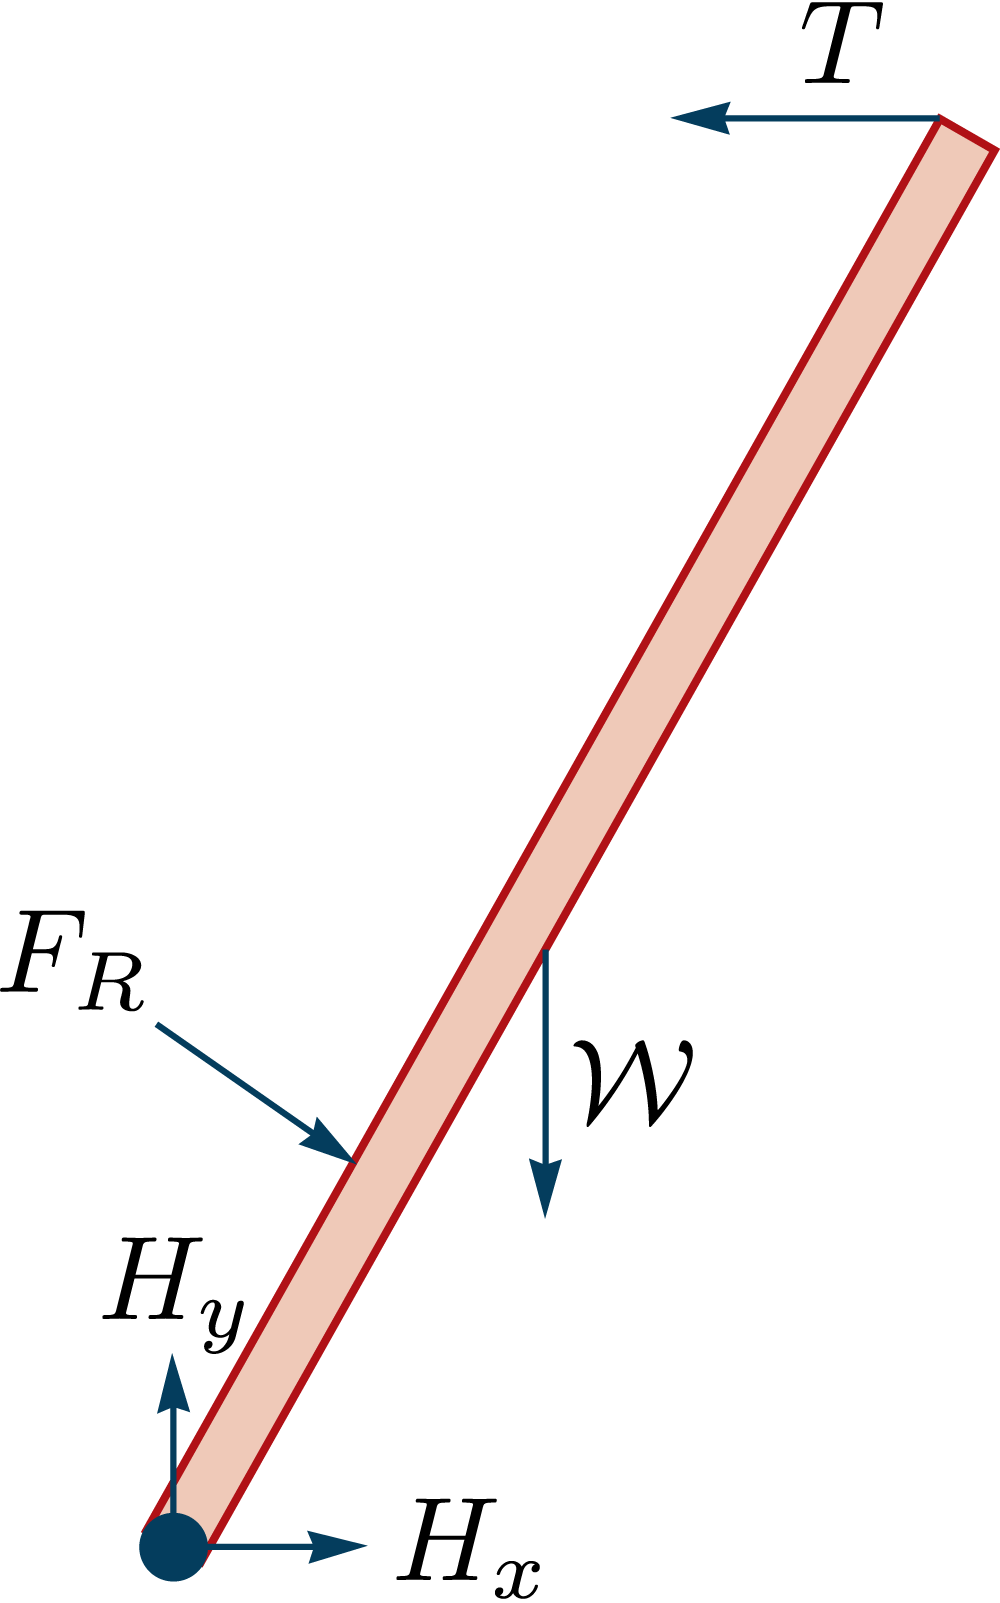
\includegraphics[width=0.2\textwidth]{2-8-3_1.png}
\end{center}
At equilibrium,
\[
\sum M_H=0
\]
\[
0=T(L_1\sin\theta)-\mathcal{W}\left(\frac{L_1}{2}\cos\theta\right)-F_R(L_2-y_R)
\]
Thus,
\[
T(L_1\sin\theta)=\mathcal{W}\left(\frac{L_1}{2}\cos\theta\right)+F_R(L_2-y_R)
\]
\[
T=\frac{\mathcal{W}\left(\frac{L_1}{2}\cos\theta\right)+F_R(L_2-y_R)}{L_1\sin\theta}
\]
\[
=\frac{(800\ \mathrm{lb})\left(\frac{8\ \mathrm{ft}}{2}\cos58^\circ\right)+(2850\ \mathrm{lb})(6\ \mathrm{ft}-4.00\ \mathrm{ft})}{(8\ \mathrm{ft})\sin58^\circ}
\]
\[
\boxed{T=1090\ \mathrm{lb}}
\]
\end{itemize}


\textbf{Problem 2.8.4}\\
An image of a dam is shown below. The headwater side of the dam has height $h_H=99\ \mathrm{ft}$, and the tailwater side of the dam has height $h_T=29\ \mathrm{ft}$. Consider a unit length of the dam $(b=1\ \mathrm{ft})$, assume the slope of the inclined wall is $0.65$ to $1.0$, and assume $\gamma=62.4\ \mathrm{lb/ft^3}$.
\begin{center}
    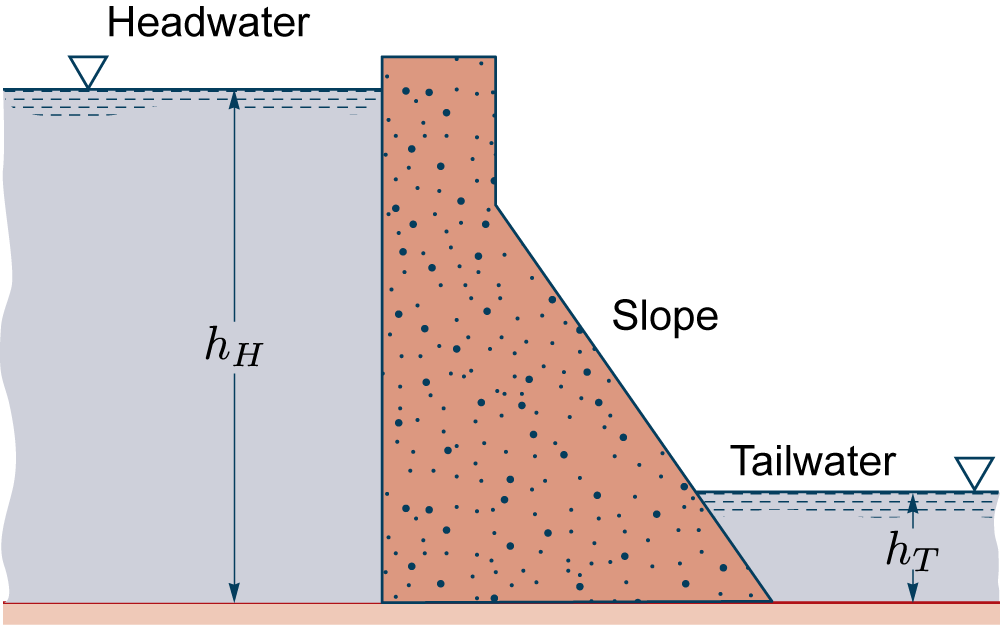
\includegraphics[width=0.5\textwidth]{2-8-4.png}
\end{center}
\begin{itemize}
\item[(a)] Determine the magnitude of the hydrostatic force acting on the headwater vertical wall of the dam.
\item[(b)] Determine the location of the hydrostatic force acting on the headwater vertical wall of the dam.
\item[(c)] Determine the magnitude of the hydrostatic force acting on the tailwater inclined wall and the location of this force.
\end{itemize}
\textbf{Solution}
\begin{itemize}
\item[(a)] The resultant force on the headwater vertical wall acts as shown below.
\begin{center}
    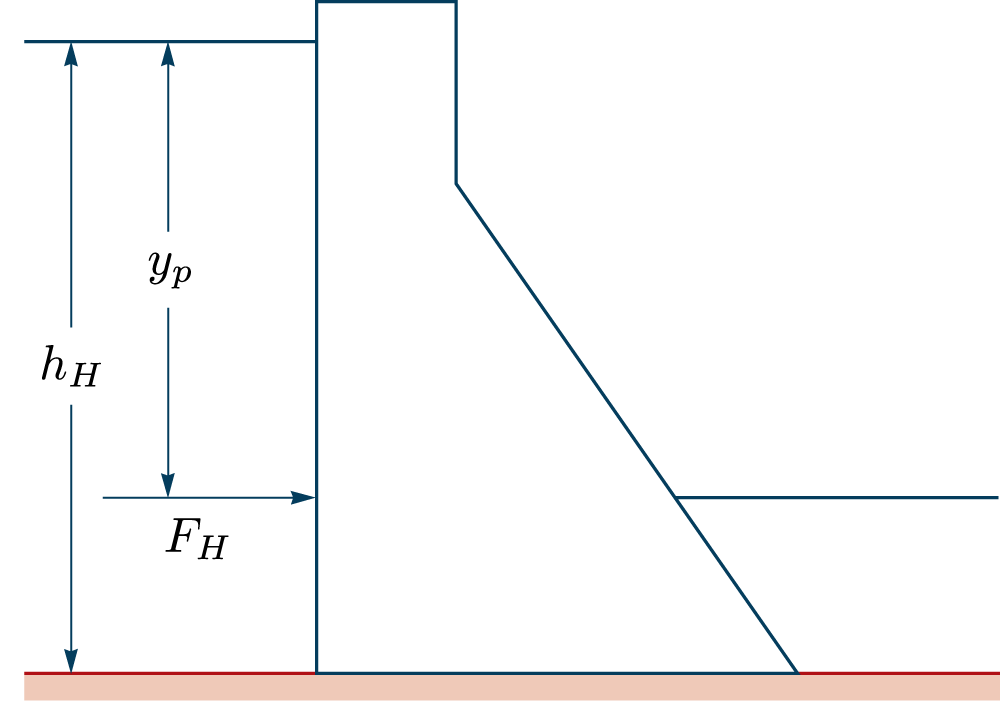
\includegraphics[width=0.4\textwidth]{2-8-4a_1.png}
\end{center}
The vertical distance from the fluid surface to the centroid of the area is
\[
h_c=\frac{h_H}{2}
=\frac{99\ \mathrm{ft}}{2}
=49.5\ \mathrm{ft}
\]
Thus, the magnitude of the resultant force is
\[
F_H=\gamma h_cA
\]
\[
=\left(62.4\ \mathrm{lb/ft^3}\right)(49.5\ \mathrm{ft})[(1\ \mathrm{ft})(99\ \mathrm{ft})]
\]
\[
\boxed{F_H=306000\ \mathrm{lb}}
\]

\item[(b)] The second moment of area is
\[
I_{xc}=\frac{1}{12}ba^3
\]
\[
=\frac{1}{12}(1\ \mathrm{ft})(99\ \mathrm{ft})^3
=80900\ \mathrm{ft^4}
\]
Thus, the location of the resultant force is
\[
y_p=\frac{I_{xc}}{y_cA}+y_c
\]
\[
=\frac{80900\ \mathrm{ft^4}}{(49.5\ \mathrm{ft})[(1\ \mathrm{ft})(99\ \mathrm{ft})]}+49.5\ \mathrm{ft}
\]
\[
\boxed{y_p=66.0\ \mathrm{ft}}
\]

\item[(c)] The resultant force on the tailwater inclined wall acts as shown below.
\begin{center}
    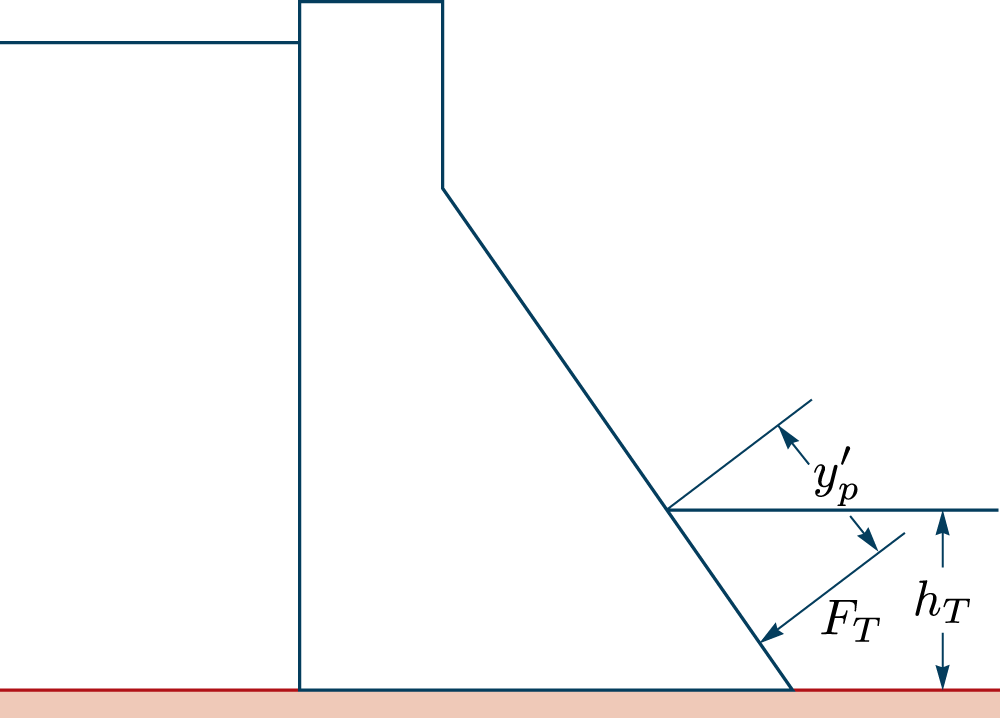
\includegraphics[width=0.4\textwidth]{2-8-4b_1.png}
\end{center}
The length of the inclined submerged surface is
\[
a=29\ \mathrm{ft}\left(\frac{\sqrt{1.0^2+0.65^2}}{1.0}\right)
\]
so the area is
\[
A=ba
=(1\ \mathrm{ft})\left[29\ \mathrm{ft}\left(\frac{\sqrt{1.0^2+0.65^2}}{1.0}\right)\right]
=34.6\ \mathrm{ft^2}
\]
The centroid depth is
\[
h_c=\frac{h_T}{2}
=\frac{29\ \mathrm{ft}}{2}
=14.5\ \mathrm{ft}
\]
Thus,
\[
F_T=\gamma h_cA
\]
\[
=\left(62.4\ \mathrm{lb/ft^3}\right)\left(\frac{29\ \mathrm{ft}}{2}\right)(34.6\ \mathrm{ft^2})
\]
\[
\boxed{F_T=31300\ \mathrm{lb}}
\]
The second moment of area is
\[
I_{xc}=\frac{1}{12}ba^3
\]
\[
=\frac{1}{12}(1\ \mathrm{ft})\left[29\ \mathrm{ft}\left(\frac{\sqrt{1.0^2+0.65^2}}{1.0}\right)\right]^3
\]
\[
=3450\ \mathrm{ft^4}
\]
The centroid coordinate along the inclined surface is
\[
y_c=\frac{a}{2}
=\frac{34.6\ \mathrm{ft}}{2}
=17.3\ \mathrm{ft}
\]
Thus, the location of the resultant force is
\[
y_p'=\frac{I_{xc}}{y_cA}+y_c
\]
\[
=\frac{3450\ \mathrm{ft^4}}{(17.3\ \mathrm{ft})(34.6\ \mathrm{ft^2})}+17.3\ \mathrm{ft}
\]
\[
\boxed{y_p'=23.1\ \mathrm{ft}}
\]
\end{itemize}

\section*{\fbox{2.10: Hydrostatic force on a curved surface}}
\textbf{Problem 2.10.1}\\
The figure below shows a cross section of a submerged tunnel used by automobiles to travel under a river. The depth from the free surface of the river to the top of the tunnel is $h=28\ \mathrm{ft}$. The tunnel has a radius of $R=23\ \mathrm{ft}$ and is $2.0$ mi long. Assume $\gamma=62.4\ \mathrm{lb/ft^3}$.
\begin{center}
    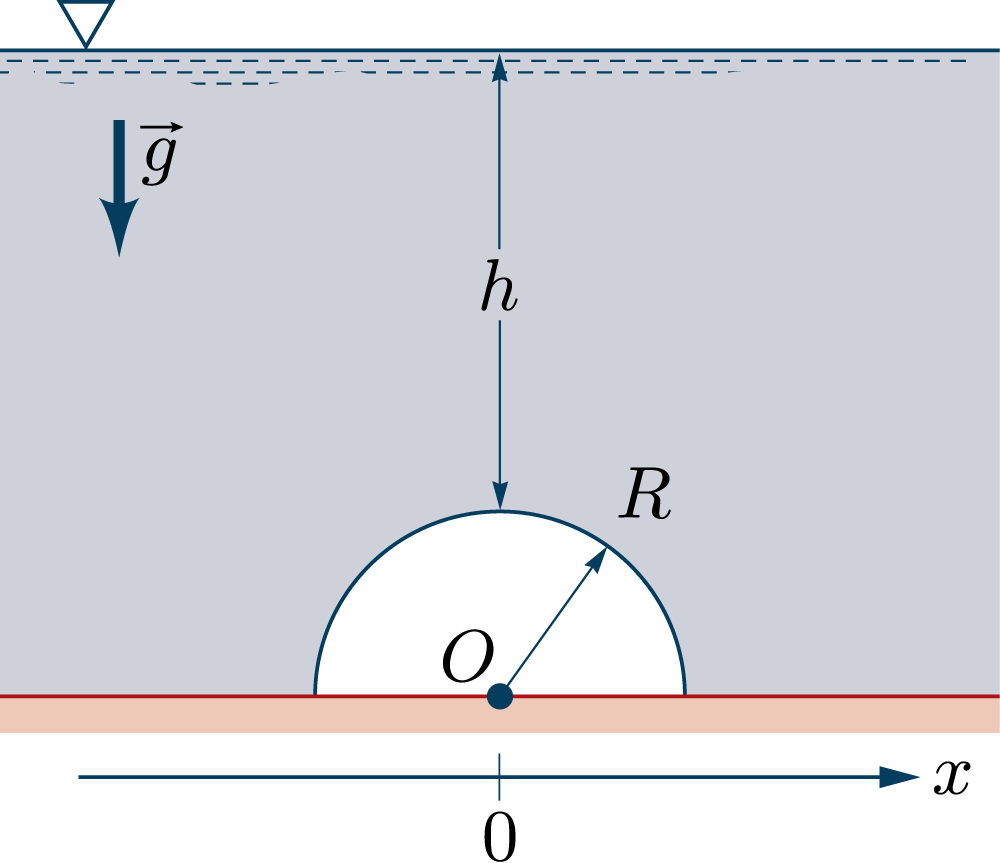
\includegraphics[width=0.5\textwidth]{2-10-1.png}
\end{center}
\begin{itemize}
\item[(a)] Find the magnitude of the resultant hydrostatic force on the circular roof of the tunnel.
\item[(b)] Find the location of the resultant hydrostatic force on the circular roof of the tunnel, assuming point $O$ is at the origin.
\end{itemize}
\textbf{Solution}
\begin{itemize}
\item[(a)] Due to symmetry, there is no net horizontal force on the roof. The vertical force is equal to the weight of fluid above the tunnel and acts through the centroid of the fluid volume. Let $l$ be the length of the tunnel. Then,
\[
F=\gamma V
=\gamma l\left[2R(h+R)-\frac{\pi}{2}R^2\right]
\]
\[
=\left(62.4\ \mathrm{lb/ft^3}\right)\left[(2.0\ \mathrm{mi})\left(\frac{5280\ \mathrm{ft}}{1\ \mathrm{mi}}\right)\right]
\left[2(23\ \mathrm{ft})(28\ \mathrm{ft}+23\ \mathrm{ft})-\frac{\pi}{2}(23\ \mathrm{ft})^2\right]
\]
\[
\boxed{F=9.98\times10^8\ \mathrm{lb}}
\]
\item[(b)] The force acts downward through point $O$ due to symmetry. Thus,
\[
\boxed{x=0\ \mathrm{ft}}
\]
\end{itemize}
\textbf{Problem 2.10.2}\\
A plug in the bottom of a pressurized tank is conical in shape, as shown in the figure below. The air gage pressure is $40\ \mathrm{kPa}$, and the liquid in the tank has a specific weight of $27\ \mathrm{kN/m^3}$. Assume $h=3.6\ \mathrm{m}$. The cone has a height of $1\ \mathrm{m}$ and an included angle of $60^\circ$.
\begin{center}
    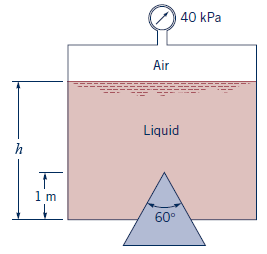
\includegraphics[width=0.5\textwidth]{2-10-2.png}
\end{center}
\begin{itemize}
\item[(a)] Determine the magnitude of the force exerted on the curved surface of the cone within the tank due to the $40\ \mathrm{kPa}$ pressure and the liquid.
\item[(b)] Determine the direction of the force exerted on the curved surface of the cone.
\item[(c)] Determine the line of action of the force exerted on the curved surface of the cone.
\end{itemize}
\textbf{Solution}
\begin{itemize}
\item[(a)] The forces acting on the cone are shown in the free-body diagram below.
\begin{center}
    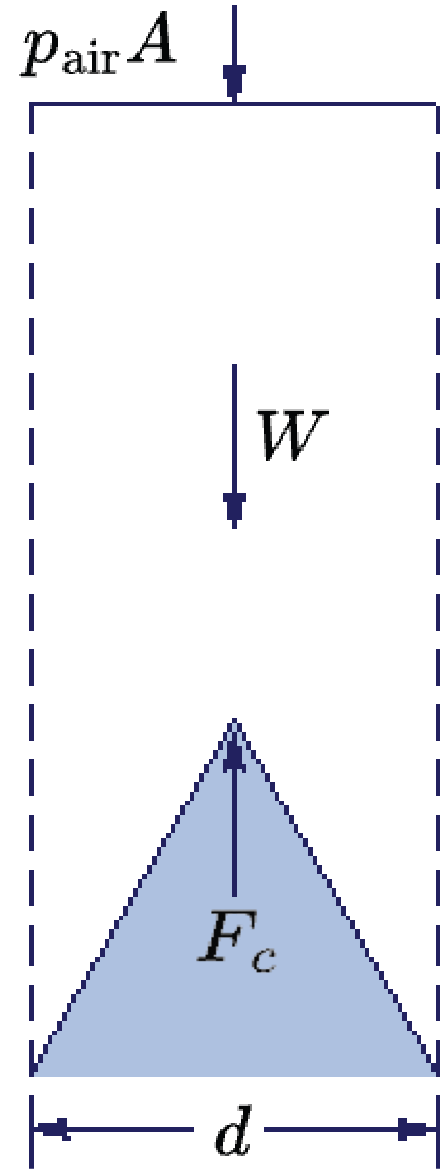
\includegraphics[width=0.15\textwidth]{2-10-2_1.png}
\end{center}
From the cone geometry,
\[
\tan30^\circ=\frac{d/2}{1}
\]
\[
d=2\tan30^\circ=1.155\ \mathrm{m}
\]
The volume of the cone is
\[
V_{\mathrm{cone}}=\frac{\pi}{3}\left(\frac{d}{2}\right)^2(1)
\]
For vertical equilibrium,
\[
\sum F_{\mathrm{vertical}}=0
\]
so
\[
F_c=p_{\mathrm{air}}A+W
\]
where $F_c$ is the force exerted by the cone on the fluid. The force due to the air pressure is
\[
p_{\mathrm{air}}A
=(40\ \mathrm{kPa})\left(\frac{\pi}{4}d^2\right)
\]
\[
=(40\ \mathrm{kPa})\left(\frac{\pi}{4}\right)(1.155\ \mathrm{m})^2
=41.9\ \mathrm{kN}
\]
The weight of the fluid above the cone is
\[
W=\gamma\left[\frac{\pi}{4}d^2(3.6\ \mathrm{m})-\frac{\pi}{3}\left(\frac{d}{2}\right)^2(1\ \mathrm{m})\right]
\]
\[
=\gamma\pi d^2\left[\frac{3.6\ \mathrm{m}}{4}-\frac{1\ \mathrm{m}}{12}\right]
\]
\[
=\left(27\ \mathrm{kN/m^3}\right)\pi(1.155\ \mathrm{m})^2(0.817\ \mathrm{m})
=92.4\ \mathrm{kN}
\]
Thus,
\[
F_c=41.9\ \mathrm{kN}+92.4\ \mathrm{kN}
\]
\[
\boxed{F_c=134\ \mathrm{kN}}
\]
\item[(b)] The force exerted on the cone is
\[
\boxed{\text{vertically downward}}
\]
\item[(c)] By symmetry, all horizontal force components cancel. Therefore, the resultant force acts
\[
\boxed{\text{along the cone axis}}
\]
\end{itemize}
\section*{\fbox{2.11 Buoyancy, flotation, and stability}}
\textbf{Problem 2.11.1}\\
A $1$-ft-diameter, $2$-ft-long cylinder floats in an open tank containing a liquid having a specific weight $\gamma$. A U-tube manometer is connected to the tank, as shown in the figure below. When the pressure in pipe $A$ is $0.15\ \mathrm{psi}$ below atmospheric pressure, the various fluid levels are as shown. For the gage fluid, $SG=1.4$. Determine the weight of the cylinder. Note that the top of the cylinder is flush with the fluid surface.
\begin{center}
    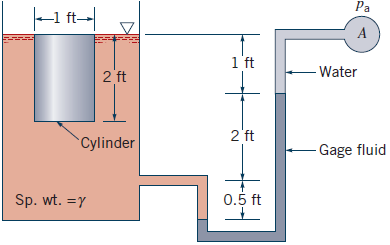
\includegraphics[width=0.5\textwidth]{2-11-1.png}
\end{center}
\textbf{Solution}
\begin{itemize}
\item A free-body diagram of the cylinder is shown below.
\begin{center}
    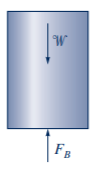
\includegraphics[width=0.15\textwidth]{2-11-1_1.png}
\end{center}
\item From vertical equilibrium,
\[
\sum F_{\mathrm{vertical}}=0
\]
\[
\mathcal{W}=F_B
=\gamma\left(\frac{\pi}{4}\right)(1\ \mathrm{ft})^2(2\ \mathrm{ft})
=\frac{\pi\gamma}{2}
\]
\item Applying the manometer equation,
\[
\gamma(3.5\ \mathrm{ft})
-SG\,\gamma_{\mathrm{H_2O}}(2.5\ \mathrm{ft})
-\gamma_{\mathrm{H_2O}}(1\ \mathrm{ft})
=p_a
\]
\[
\gamma(3.5\ \mathrm{ft})
-(1.4)\left(62.4\ \mathrm{lb/ft^3}\right)(2.5\ \mathrm{ft})
-\left(62.4\ \mathrm{lb/ft^3}\right)(1\ \mathrm{ft})
=\left(-0.15\ \mathrm{lb/in.^2}\right)\left(\frac{144\ \mathrm{in.^2}}{1\ \mathrm{ft^2}}\right)
\]
\item Solving for the specific weight,
\[
\gamma=
\frac{
\left(-0.15\ \mathrm{lb/in.^2}\right)\left(\frac{144\ \mathrm{in.^2}}{1\ \mathrm{ft^2}}\right)
+(1.4)\left(62.4\ \mathrm{lb/ft^3}\right)(2.5\ \mathrm{ft})
+\left(62.4\ \mathrm{lb/ft^3}\right)(1\ \mathrm{ft})
}{
3.5\ \mathrm{ft}
}
\]
\[
\gamma=74.1\ \mathrm{lb/ft^3}
\]
\item Therefore,
\[
\mathcal{W}
=\left(\frac{\pi}{2}\ \mathrm{ft^3}\right)\left(74.1\ \mathrm{lb/ft^3}\right)
\]
\[
\boxed{\mathcal{W}=116\ \mathrm{lb}}
\]
\end{itemize}

\section*{\fbox{2.12: Pressure variation in a fluid with rigid-body motion}}
\textbf{Problem 2.12.1}\\
An open, $1.8$-ft-diameter tank contains water to a depth of $3.7\ \mathrm{ft}$ when at rest. If the tank is rotated about its vertical axis with an angular velocity of $159\ \mathrm{rev/min}$, determine the minimum height of the tank walls to prevent water from spilling over the sides.
\begin{center}
    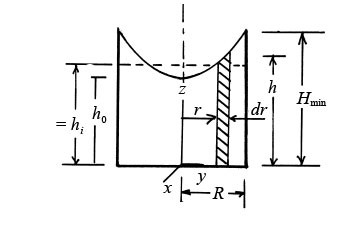
\includegraphics[width=0.5\textwidth]{2-12-1.jpg}
\end{center}
\textbf{Solution}
\begin{itemize}
\item For a free surface,
\[
z=\frac{\omega^2r^2}{2g}+\text{constant}
\]
which can be rewritten as
\[
h=\frac{\omega^2r^2}{2g}+h_0
\]
\item The volume of fluid in the rotating tank is
\[
V_f=\int_0^R 2\pi r h\,dr
\]
\[
=2\pi\int_0^R\left(\frac{\omega^2r^3}{2g}+h_0r\right)dr
\]
\[
=\frac{\pi\omega^2R^4}{4g}+\pi h_0R^2
\]
\[
=\frac{\pi\left(159\ \mathrm{rev/min}\times\frac{2\pi\ \mathrm{rad}}{1\ \mathrm{rev}}\times\frac{1\ \mathrm{min}}{60\ \mathrm{s}}\right)^2(0.9\ \mathrm{ft})^4}{4(32.2\ \mathrm{ft/s^2})}+\pi h_0(0.9\ \mathrm{ft})^2
\]
\[
=\pi(1.41+0.810h_0)\ \mathrm{ft^3}
\]
\item Since the initial volume is
\[
V_i=\pi R^2h_i
=\pi(0.9\ \mathrm{ft})^2(3.7\ \mathrm{ft})
=3.00\pi\ \mathrm{ft^3}
\]
and the final volume must be equal to the initial volume,
\[
V_f=V_i
\]
\[
\pi(1.41+0.810h_0)=3.00\pi
\]
\[
h_0=1.96\ \mathrm{ft}
\]
\item Thus, from the free-surface equation,
\[
h_{\min}=\frac{\omega^2R^2}{2g}+h_0
\]
\[
=\frac{\left(159\ \mathrm{rev/min}\times\frac{2\pi\ \mathrm{rad}}{1\ \mathrm{rev}}\times\frac{1\ \mathrm{min}}{60\ \mathrm{s}}\right)^2(0.9\ \mathrm{ft})^2}{2(32.2\ \mathrm{ft/s^2})}+1.96\ \mathrm{ft}
\]
\[
\boxed{h_{\min}=5.44\ \mathrm{ft}}
\]
\end{itemize}
\textbf{Problem 2.12.2}\\
A $3$-gal cylindrical open container with a bottom area of $130\ \mathrm{in.^2}$ is filled with water and rests on the floor of an elevator. Note $1\ \mathrm{gal}=231\ \mathrm{in.^3}$ and $\rho_{\mathrm{water}}=1.94\ \mathrm{slugs/ft^3}$.
\begin{itemize}
\item[(a)] Determine the fluid pressure at the bottom of the container when the elevator has an upward acceleration of $2.3\ \mathrm{ft/s^2}$.
\item[(b)] Determine the resultant force that the container exerts on the floor of the elevator when the elevator has an upward acceleration of $2.3\ \mathrm{ft/s^2}$. The weight of the container is negligible.
\end{itemize}
\textbf{Solution}
\begin{itemize}
\item The container containing water is shown below.
\begin{center}
    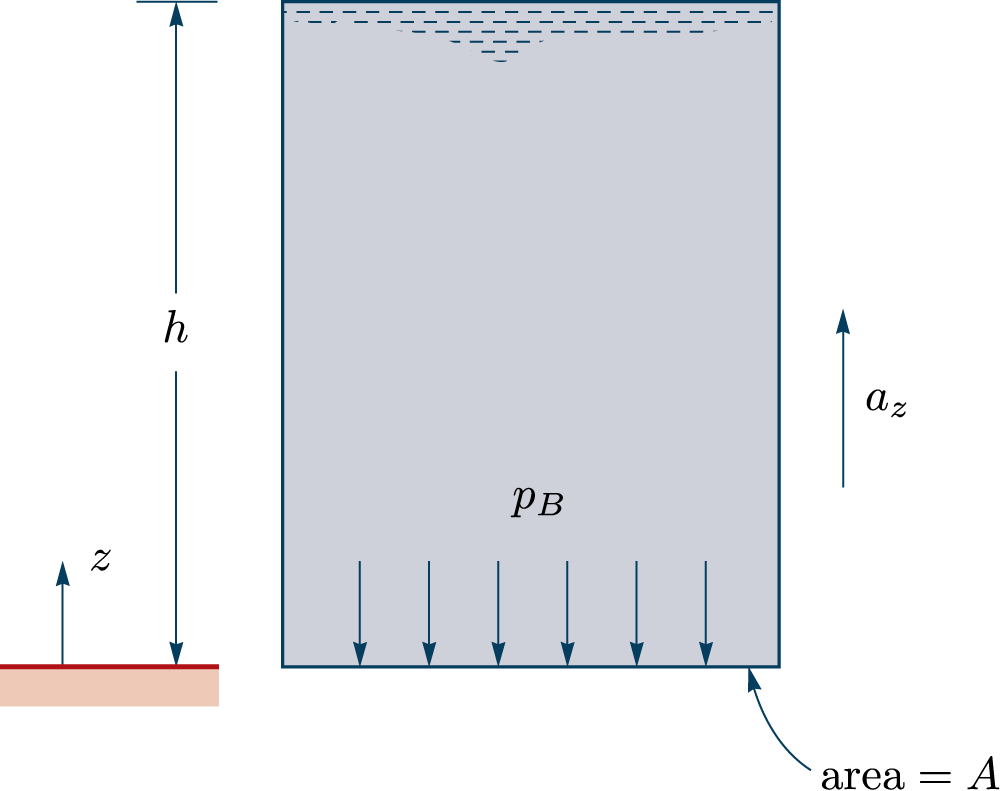
\includegraphics[width=0.4\textwidth]{2-12-2_1.png}
\end{center}
\item The height $h$ of the container is calculated using the volume and area of the container,
\[
Ah=V
\]
\[
h(130\ \mathrm{in.^2})=(3\ \mathrm{gal})\left(\frac{231\ \mathrm{in.^3}}{1\ \mathrm{gal}}\right)
\]
\[
h=5.33\ \mathrm{in.}
\]
\item[(a)] Since the container is accelerating in the vertical direction, the pressure distribution is
\[
\frac{dp}{dz}=-\rho(g+a_z)
\]
Thus,
\[
\int_0^{p_B}dp=-\rho(g+a_z)\int_h^0dz
\]
and
\[
p_B=\rho(g+a_z)h
\]
\[
=\left(1.94\ \mathrm{slugs/ft^3}\right)
\left(32.2\ \mathrm{ft/s^2}+2.3\ \mathrm{ft/s^2}\right)
\left[(5.33\ \mathrm{in.})\left(\frac{1\ \mathrm{ft}}{12\ \mathrm{in.}}\right)\right]
\]
\[
=29.7\ \mathrm{slugs/(ft\cdot s^2)}
\left(\frac{1\ \mathrm{lb}}{1\ \mathrm{slug\cdot ft/s^2}}\right)
\]
\[
\boxed{p_B=29.7\ \mathrm{lb/ft^2}}
\]
\item[(b)] The free-body diagram of the container is shown below.
\begin{center}
    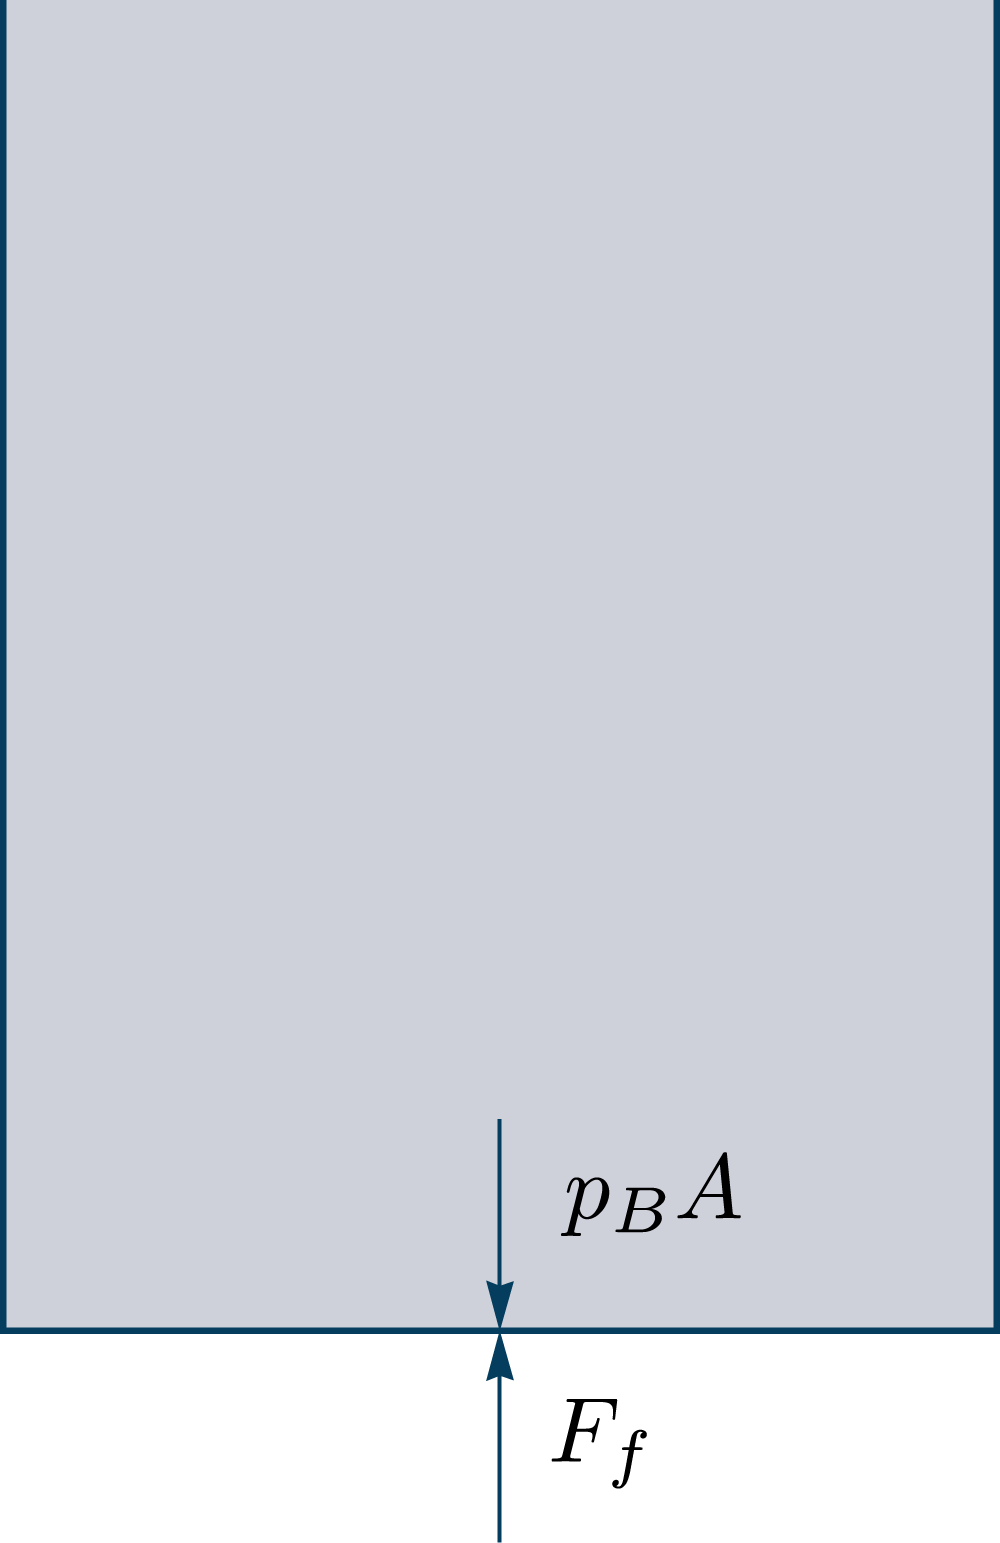
\includegraphics[width=0.2\textwidth]{2-12-2_2.png}
\end{center}
From the free-body diagram,
\[
F_f=p_BA
\]
\[
=\left(29.7\ \mathrm{lb/ft^2}\right)(130\ \mathrm{in.^2})
\left(\frac{1\ \mathrm{ft}}{12\ \mathrm{in.}}\right)^2
\]
\[
\boxed{F_f=26.8\ \mathrm{lb}}
\]
Thus, the force of the container on the floor is $26.8\ \mathrm{lb}$ downward.
\end{itemize}

\textbf{Problem 2.12.3}\\
A closed, $0.1$-m-diameter cylindrical tank is completely filled with oil $(SG=0.9)$ and rotates about its vertical longitudinal axis with an angular velocity of $34\ \mathrm{rad/s}$. Determine the difference in pressure just under the vessel cover between a point on the circumference and a point on the axis.
\begin{center}
    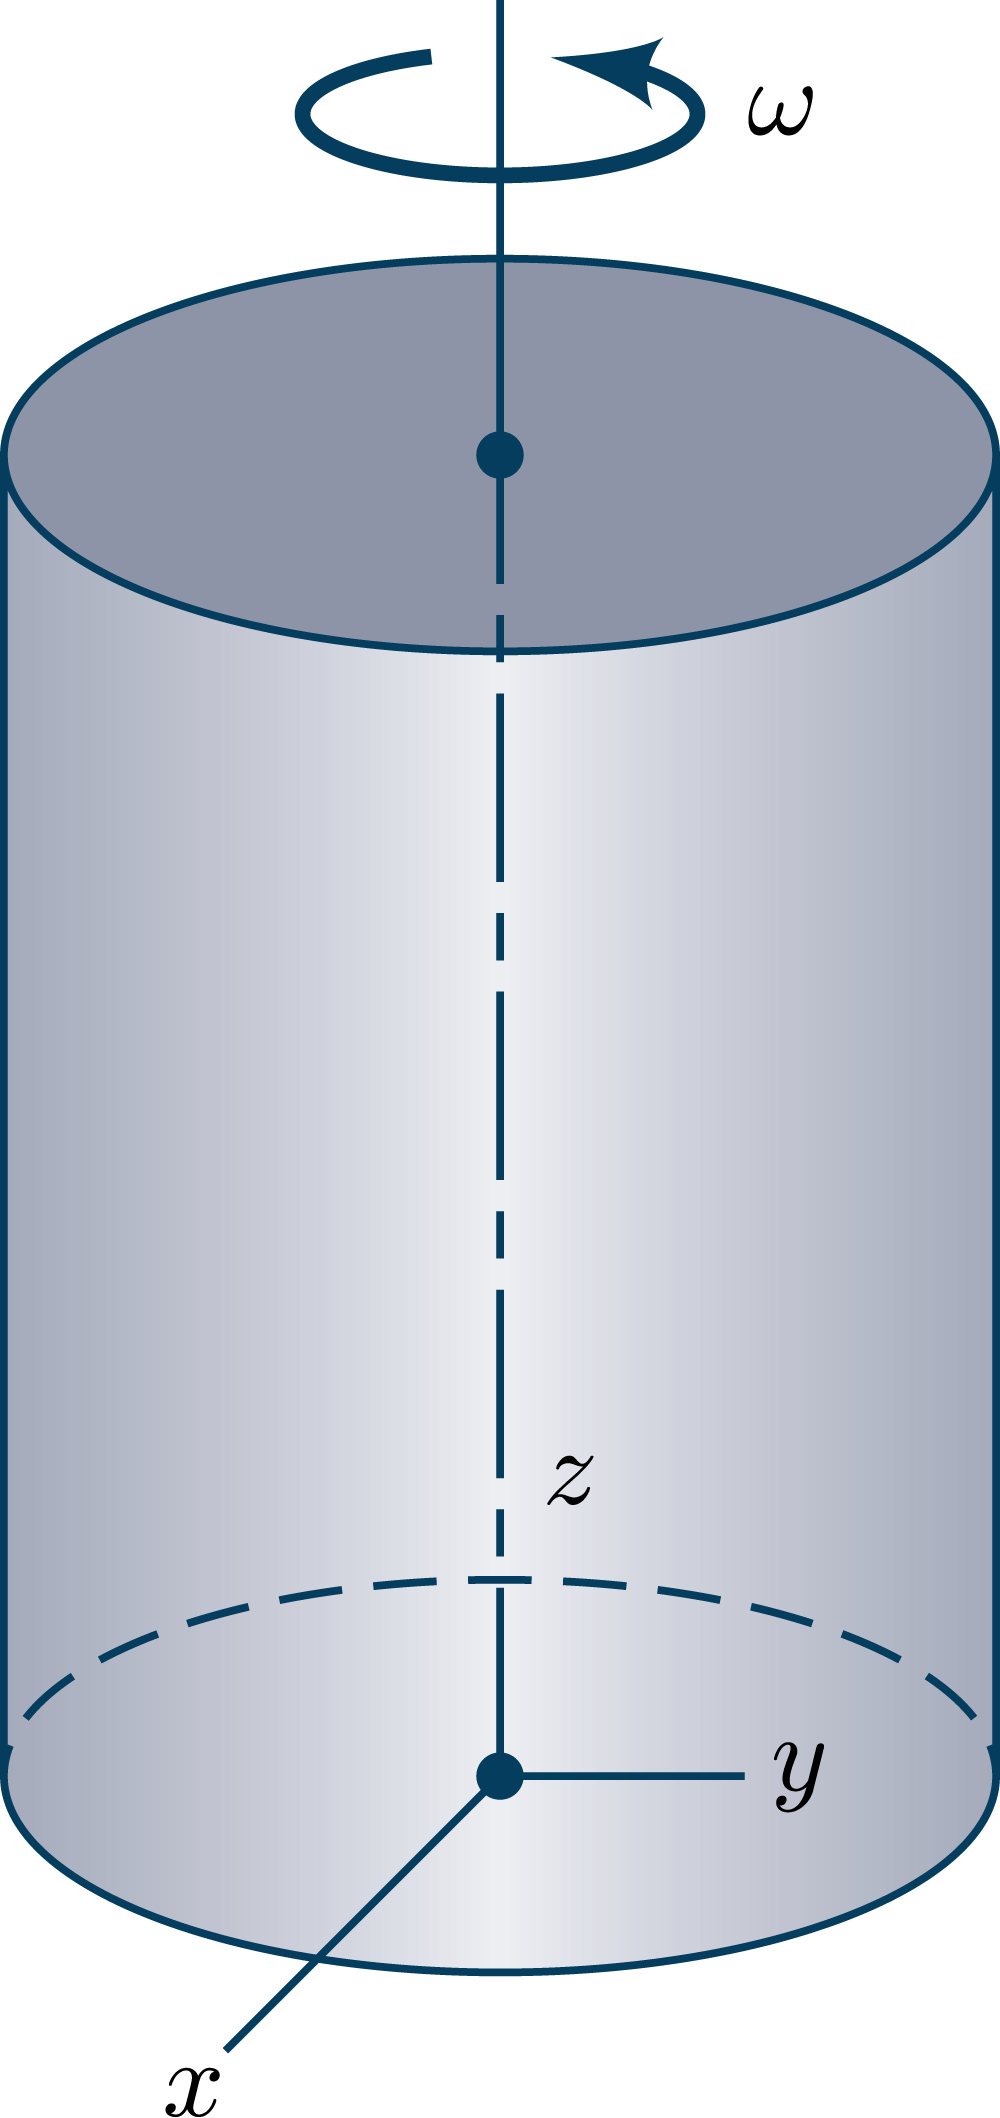
\includegraphics[width=0.2\textwidth]{2-12-3.png}
\end{center}
\textbf{Solution}
\begin{itemize}
\item The rotating cylindrical tank is shown below, where the point on the axis is labeled $A$ and the point on the circumference is labeled $B$.
\begin{center}
    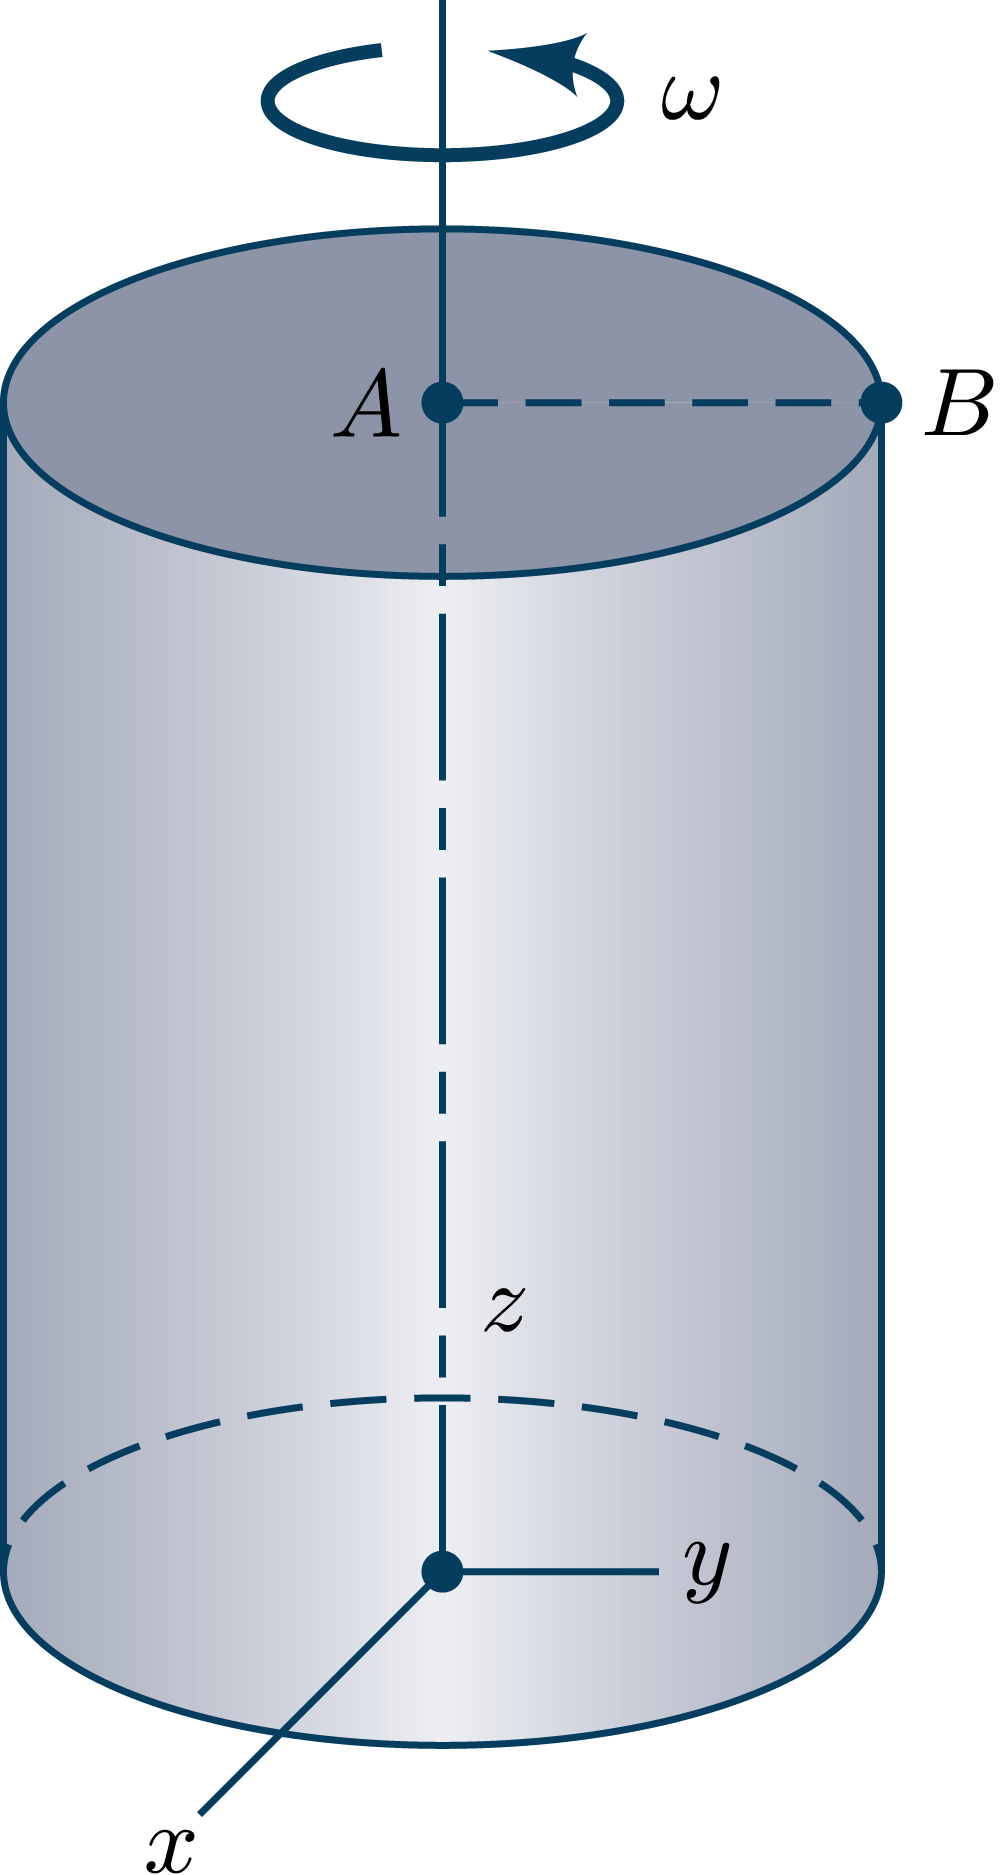
\includegraphics[width=0.2\textwidth]{2-12-3_1.png}
\end{center}
\item Pressure in the rotating fluid varies according to
\[
p=\frac{\rho\omega^2r^2}{2}-\gamma z+\text{constant}
\]
\item Since $z_A=z_B$,
\[
p_B-p_A=\frac{\rho\omega^2}{2}\left(r_B^2-r_A^2\right)
\]
\[
=\frac{[(SG)(\rho_{\mathrm{water}})]\omega^2}{2}\left(r_B^2-r_A^2\right)
\]
\[
=\frac{[(0.9)(1000\ \mathrm{kg/m^3})](34\ \mathrm{rad/s})^2}{2}
\left[\left(\frac{0.1\ \mathrm{m}}{2}\right)^2-0\right]
\]
\[
\boxed{\Delta p=1.30\ \mathrm{kPa}}
\]
\end{itemize}
\end{document}
